% This is LLNCS.DEM the demonstration file of
% the LaTeX macro package from Springer-Verlag
% for Lecture Notes in Computer Science,
% version 2.4 for LaTeX2e as of 16. April 2010
%
\documentclass{llncs}
%
\usepackage{comment}
\usepackage{mathpartir}
\usepackage{listings}
\usepackage{alltt}
\usepackage{graphicx}
\usepackage{amssymb}

%%
%% STANDARD SMC CUSTOMIZATION

% This is my comments.  The color and text style means it
% came from Eric Mercer.
% I am including 2 versions:
%   a) includes my comments in the final document
%   b) excludes my comments in the final document
\usepackage{color}
\definecolor{egmcolor}{rgb}{1.0,0.0,0.722}
\newcommand*{\egm}[1]%
%%
%% a)
{\textcolor{egmcolor}{\noindent\textbf{[egm:~}\textit{#1}]}}
%%
% Other things...
\newcommand{\figref}[1]{Figure~\ref{#1}}
\newcommand{\defref}[1]{Definition~\ref{#1}}
\newcommand{\secref}[1]{Section~\ref{#1}}
\newcommand{\lemmaref}[1]{Lemma~\ref{#1}}

%
\begin{document}
%
\pagestyle{headings}  % switches on printing of running heads%
%
\title{Proving MCAPI Executions are Correct}
\subtitle{Applying SMT Technology to Message Passing}
%\titlerunning{SMT for MCAPI Executions}

\author{Yu Huang \and Eric Mercer \and Jay McCarthy \thanks{Special thanks to Christopher Fischer, formally at BYU and now at Amazon}}
%\authorrunning{Y.~Huang \and E.~Mercer \and J.~McCarthy}
\institute{Brigham Young University \\
            \email{\{yuHuang,egm,jay\}@byu.edu}}

\maketitle

% Macros for specifying the trace-language
%% Commands For the syntax EBNF
\newcommand{\cfgnt}[1]{\emph{#1}}
\newcommand{\cfgq}[1]{\texttt{#1}}
\newcommand{\cfgt}[1]{\textbf{#1}}
\newcommand{\cfglhs}[1]{\cfgnt{#1} & $::=$}
\newcommand{\cfgrule}[2]{\cfglhs{#1} & #2 \\}
\newcommand{\cfgor}{\textbar\ }
\newcommand{\cfgstart}{\begin{tabular}{r@{\hspace{1mm}}r@{\hspace{2mm}}l}}
\newcommand{\cfgend}{\end{tabular}}
\newcommand{\cfgline}[1]{ ~ && #1 \\ }
\newcommand{\cfglinetab}[1]{ ~ && \hspace{1cm} #1 \\ }
\newcommand{\cfgorline}[1]{ ~ & \cfgor & #1 \\ }
\newcommand{\lp}{\cfgq{(}}
\newcommand{\rp}{\cfgq{)}}
\newcommand{\lb}{\cfgq{[}}
\newcommand{\rb}{\cfgq{]}}


%
%
\begin{abstract}
%% Should be 70-150 words
Asynchronous message passing for C language is an important paradigm in writing
applications for embedded heterogeneous multicore systems.  The
Multicore Association (MCA), an industry consortium promoting
multicore technology, is working to standardize message passing into a
single API, MCAPI, for bare metal implementation and portability
across platforms.  Correctness in such an API is difficult to reason
about manually, and testing against reference solutions is equally
difficult as reference solutions implement an unknown set of allowed
behaviors, and programmers have no way to directly control API
internals to expose or reproduce errors.  This paper encodes an MCAPI
execution as an SMT problem, which if satisfiable, yields a feasible
execution schedule on the same trace,
such that it resolves non-determinism in the MCAPI runtime in the way that it now fails user provided assertions.
Such an encoding is useful for test, debug, and
verification of MCAPI program execution.  The novelty in the encoding
is the use of match pairs (potential send and receive couplings) to
model the MCAPI execution in the SMT problem.  Match-pair encoding for
MCAPI executions, when compared to other encoding strategies, is
simpler to reason about, results in significantly fewer terms in the
SMT problem, and captures feasible behaviors that are ignored in
previously published techniques. To our knowledge, this is the first SMT encoding of MCAPI application that is able to run in \textit{infinite-buffer} semantics, meaning that more messages can be received by a particular endpoint at a time. In other words, our encoding with infinite-buffer controls more non-deterministic behaviors at runtime. Our results demonstrate that our SMT encoding reduces $66\%$ to $80\%$ the size of that of the existing technology. In addition, our encoding runs average eight times faster and uses two times less memory than the existing technology on the benchmarks in our experiment.


\keywords{Abstraction, refinement, SMT, message passing}
\end{abstract}
%
\section{Introduction}
Embedded devices fill all sorts of crucial roles in our lives. They exist as
medical devices, as network infrastructure, and they control our automobiles.
Embedded devices continue to become more powerful as computing hardware becomes
smaller and more modular. It is now becoming commonplace to find multiple
processing units inside a single device. The Multicore Association (MCA) is an
industry group that has formed to define specifications for low-level
communication, resource management, and task management for embedded heterogeneous
multicore devices \cite{mca}.

One specification that the MCA has released is the Multicore
Association Communications API (MCAPI) \cite{mcapi}. The specification
defines types and functions for simple message passing operations between different
computing entities within a device. Messages can be passed across
persistent channels that force an ordering of the messages, or they
can be passed to specific \emph{endpoints} within the system. The
specification places few ordering constraints on messages passed from
one endpoint to another. This freedom introduces the possibility of a race between multiple messages to common endpoints thus giving rise to non-deterministic behavior in the runtime\ \cite{netzer:spdt96}. If an
application has non-determinism, it is not possible
to test and debug such an application without a way to directly (or
indirectly) control the MCAPI runtime.

There are two ways to implement the MCAPI semantics: infinite-buffer
semantics (the message is copied into a runtime buffer on the API
call) and zero-buffer semantics (the message has no buffering)
\cite{sarvani:fm09}.  An infinite-buffer semantics provides more
non-deterministic behaviors in matching send and receives because the
runtime can arbitrarily delay a send to create interesting (and
unexpected) send reorderings. The zero-buffer semantics follow
intuitive message orderings as a send and receive essentially
rendezvous.

Sharma et al. propose a method to indirectly control the MCAPI runtime
to verify MCAPI programs under zero-buffer semantics
\cite{sharma:fmcad09}. As the work does not address infinite-buffer
semantics, it is somewhat limited in its application. The work does
provide a dynamic partial order reduction for the model checker, but
such a reduction is not sufficient to control state space explosion in
the presence of even moderate non-determinism between message sends
and receives. A key insight from the approach is its direct use of
match pairs--couplings for potential sends and receives.

Wang \textit{et al.} propose an alternative method for resolving
non-determinism for program verification using symbolic methods in the context
of shared memory systems \cite{wang:fse09}. The work observes a
program trace, builds a partial order from that trace called a
concurrent trace program (CTP), and then creates an SMT problem from
the CTP that if satisfied indicates a property violation. 

Elwakil \textit{et al.} extend the work of Wang \textit{et al.} to
message passing and claim the encoding supports both semantics. A
careful analysis of the encoding, however, shows it to not work under
infinite-buffer semantics and to miss behaviors under zero-buffer
semantics \cite{elwakil:padtad10}. Interestingly, the encoding assumes
the user provides a precise set of match-pairs as input with the
program trace, and it then uses those match-pairs in a non-obvious way
to constrain the happens-before relation in the encoding. The work
does not discuss how to generate the match-pairs, which is a
non-trivial input to manually generate for large or complex program
traces. An early proof claims that the problem of finding a precise
set of match-pairs given a program trace is NP-complete
\cite{match-pair-np-complete}.

\examplefigone

 This paper presents a proof that resolving non-determinism in message
 passing programs in a way that meets all assertions is
 NP-complete. The paper then presents an SMT encoding for MCAPI
 program executions that works for both zero and infinite buffer
 semantics. The encoding does require an input set of match-pairs as
 in prior work, but unlike prior work, the match-set can be
 over-approximated and the encoding is still sound and complete. The
 encoding requires fewer terms to capture all possible program
 behavior when compared to other proposed methods making it more
 efficient in the SMT solver.  To address the problem of generating
 match-pairs, an algorithm to generate the over-approximated set is
 given. To summarize, the main contributions in this paper are

\begin{enumerate}
%\item An MCAPI program that introduces non-deterministic behavior.
%\item A trace language framework that simulates and verifies an execution trace of an MCAPI program.
%\item A modified trace language framework that generates an SMT problem for a single trace in the machine executions.
\item a proof that the problem of matching sends to receives in a way that meets assertions is NP-complete;
\item a correct and efficient SMT encoding of an MCAPI program
  execution that detects all program errors under zero or infinite
  buffer semantics given the input set of potential match-pairs
  contains at least the precise set of match-pairs; and
\item an $O(N^2)$ algorithm to generate an over-approximation of
  possible match-pairs, where $N$ is the size of the execution trace
  in lines of code.
\end{enumerate}

The rest of the paper is organized as follows: Section 2 presents an
MCAPI program illustrating the non-determinism in runtime
specification. Section 3 is the proof that the problem is
NP-complete. Section 4 defines the SMT encoding using potential
math-pairs. The encoding is shown to be sound and complete even under
an over-approximated set of match-pairs. Section 5 provides a solution
to the outstanding problem of generating feasible match pairs. Section
6 presents the experimental results that show the encoding to be
efficient. Section 7 discusses related work. And Section 8 presents
conclusions and future work.


% ---------------------------------------------------------------------
% Save boxes for the various figures in the example section
% ---------------------------------------------------------------------
\newsavebox{\boxTZero}
\begin{lrbox}{\boxTZero}
\begin{minipage}[t]{0.65\linewidth}
\begin{alltt}
   00 initialize(NODE_0,&v,&s);
   01 ep0 = create_endpoint(PORT_0,&s);

04 02 msg_recv_i(ep0,A,sizeof(A),&rcvA,&s);
05 03 wait(&rcvA,&size,&s,MCAPI_INF);
06 04 a = atoi(A);

11 05 msg_recv_i(ep0,B,sizeof(B),&rcvB,&s);
12 06 wait(&rcvB,&size,&status,MCAPI_INF);
13 07 b = atoi(B);

14 08 if (b > 0)
15 09    assert(a == 4);

   10 finalize(&s);
\end{alltt}
\end{minipage}
\end{lrbox}

\newsavebox{\boxATZero}
\begin{lrbox}{\boxATZero}
\begin{minipage}[t]{0.65\linewidth}
\begin{alltt}
08 0_0         (0_0 (rcvi rcvA 0 a))
09 (0_1 (0 1)) (0_1 (wait rcvA))

10 0_2         (0_2 (rcvi rcvB 0 b))
11 (0_3 (0 2)) (0_3 (wait rcvB))

12 0_4         (0_4 (assume (> b 0)))
13 0_5         (0_5 (assert (= a 4)))
\end{alltt}
\end{minipage}
\end{lrbox}

\newsavebox{\boxTOne}
\begin{lrbox}{\boxTOne}
\begin{minipage}[t]{0.65\linewidth}
\begin{alltt}
   00 initialize(NODE_1,&v,&s);
   01 ep1 = create_endpoint(PORT_1,&s);
   02 ep0 = get_endpoint(NODE_0,PORT_0,&s);

07 03 msg_recv_i(ep1,C,sizeof(C),&rcvC,&s);
08 04 wait(&rcvC,&size,&s,INF);

09 05 msg_send_i(ep1,ep0,"1",2,N,&snd3,&s);
10 06 wait(&snd3,&size,&s,MCAPI_INF);

   07 finalize(&s);
\end{alltt}
\end{minipage}
\end{lrbox}

\newsavebox{\boxATOne}
\begin{lrbox}{\boxATOne}
\begin{minipage}[t]{0.65\linewidth}
\begin{alltt}
04 1_0         (1_0 (rcvi rcvC 1 c))
05 (1_1 (1 2)) (1_1 (wait rcvC))

06 1_2         (1_2 (sndi snd3 1 0 0x1))
07 1_3         (1_3 (wait snd3))
\end{alltt}
\end{minipage}
\end{lrbox}

\newsavebox{\boxTTwo}
\begin{lrbox}{\boxTTwo}
\begin{minipage}[t]{0.65\linewidth}
\begin{alltt}
   00 initialize(NODE_2,&v,&s);
   01 t2 = create_endpoint(PORT_2,&s);
   02 t0 = get_endpoint(NODE_0,PORT_0,&s);
   03 t1 = get_endpoint(NODE_1,PORT_1,&s);

00 04 msg_send_i(ep2,ep0,"4",2,N,&snd1,&s);
01 05 wait(&snd1,&size,&status,MCAPI_INF);

02 06 msg_send_i(ep2,ep1,"Go",3,N,&snd2,&s);
03 07 wait(&snd2,&size,&status,MCAPI_INF);
   08
   09 finalize(&s);
\end{alltt}
\end{minipage}
\end{lrbox}

\newsavebox{\boxATTwo}
\begin{lrbox}{\boxATTwo}
\begin{minipage}[t]{0.65\linewidth}
\begin{alltt}
00 2_0        (2_0 (sndi snd1 2 0 0x4))
01 2_1        (2_1 (wait snd1))

02 2_2        (2_2 (sndi snd2 2 1 0x476f00))
03 2_3        (2_3 (wait snd2))
\end{alltt}
\end{minipage}
\end{lrbox}

\newsavebox{\boxMP}
\begin{lrbox}{\boxMP}
\begin{minipage}[c]{0.2\linewidth}
\begin{alltt}
(rcvA snd1)
(rcvA snd3)

(rcvB snd1)
(rcvB snd3)

(rcvC snd2)
\end{alltt}
\end{minipage}
\end{lrbox}


\newsavebox{\boxSMT}
\begin{lrbox}{\boxSMT}
\begin{minipage}[c]{0.4\linewidth}
\begin{alltt}
(HB rcvA_loc wait_rcvA_loc)
(HB wait_rcvA_loc rcvB_loc)
(HB rcvB_loc wait_rcvB_loc)
(HB wait_rcvB_loc assume_loc)
(HB assume_loc assert_loc)
(HB rcvC_loc wait_rcvC_loc)
(HB wait_rcvC_loc snd3_loc)
(HB snd3_loc wait_snd3_loc)
(HB snd1_loc wait_snd1_loc)
(HB wait_snd1_loc snd2_loc)
(HB snd2_loc wait_snd2_loc)

(or (MATCH rcvA snd3)
    (MATCH rcvA snd1))
(or (MATCH rcvB  snd1)
    (MATCH rcvB snd3))
(NE rcvA rcvB)

(MATCH rcvC snd2)

(assert (> b 0))
(assert (not (= a 4)))
\end{alltt}
\end{minipage}
\end{lrbox}
% ---------------------------------------------------------------------
% END Save boxes
% ---------------------------------------------------------------------

\section{Example}

It is a challenge to explain intended behavior in simple scenarios
consisting of a handful of calls when dealing with concurrency. Consider
the MCAPI program in the top of \figref{fig:mcapi} that includes three
tasks that use send (\texttt{mcapi\_msg\_send\_i}) and receive
(\texttt{mcapi\_msg\_recv\_i}) calls to communicate with each other.
Line numbers appear in the second column for each task, and the
declarations of the local variables are omitted for space. Picking up
the scenario just after the endpoints are defined, lines \texttt{02}
and \texttt{05} of task 0 receive two messages on the endpoint
\textit{ep0} in variables $A$ and $B$ which are
converted to integer values and stored in variables $a$ and
$b$ on lines \texttt{04} and \texttt{07}; task 1 receives one
message on endpoint \textit{ep1} in variable \textit{C} on line
\texttt{03} and then sends the message \textit{``1''} on line \texttt{05} to
\textit{ep0}; and finally, task 2 sends messages \textit{``4''} and \textit{``Go''} on
lines \texttt{04} and \texttt{06} to endpoints \textit{ep0} and
\textit{ep1} respectively. Task 0 has additional code (lines \texttt{08} -
\texttt{10}) to assert properties of the values in $a$ and
$b$. The \texttt{mcapi\_wait} calls block until the associated
send or receive buffer is able to be used. Given the scenario, we
might ask the question: \emph{``What are the possible values of
\texttt{a} and \texttt{b} after the scenario completes?''}

Intuitively, variable \textit{a} should contain $4$ and variable
\textit{b} should contain $1$ since task 2 must first send message \textit{``4''}
to \textit{ep0} before it can send message \textit{``Go''} to \textit{ep1};
consequently, task 1 is then able to send message \textit{``1''} to
\textit{ep0}. At the end of execution the assertion on line \texttt{12}
of task 0 holds and no error is found. Such intuition is a valid
program execution, and the sequential trace (ignoring endpoint creation)
is given in the first column for each
task in \figref{fig:mcapi} starting on line \texttt{04} of task 2. This single sequential execution is not sufficient to prove correctness
however because of concurrency as other valid traces may exist. How
to test those other traces is the question answered in this paper.

A single execution through a concurrent program can be understood as a
concurrent trace program (CTP) which is a trace divided into its
concurrent components including the requisite control flow on which
the trace is valid \cite{wang:fse09}. The CTP for the trace indicated
in the first column of each task in \figref{fig:mcapi} is shown in
the bottom of the same figure. The CTP is more abstract than the
original C code, and line numbers are now grouped into a program location
(where the number in front of ``\_'' is the thread number and the number behind is the command order)
in each command, but it retains sufficient details to reason about
other possible executions. The assume statement on program location \texttt{0\_4}
of task 0 preserves the control flow of the original trace. In other
words, any alternative trace on the CTP is only valid if the assume
statement holds; otherwise, such an execution belongs to a different
path through the program. We define a trace language that takes as input a single execution trace and the CTP, to verify the correctness of executing a single trace. The trace language simulates the trace execution by rewriting the program state based on transitions described in the trace and the CTP. We apply queue movement in the language semantic to specify the communication between a send and a receive command. By applying the same framework of our trace language, an SMT problem can be defined on the simulation of a trace execution. An SMT solver for the defined problem is used to enumerate the
possible valid executions in an effort to find one that violates the
assertion on program location \texttt{0\_5} of the CTP for our example while preserving the assumption on line \texttt{0\_4}.

The novelty of the SMT encoding in this paper is its use of match
pairs rather than the state-based or order-based encoding of prior work~\cite{elwakil:padtad10,elwakil:atva10}. A match pair is the coupling of a receive to a particular send.
\figref{fig:smt}(a) is the set of possible match pairs for the CTP in
the bottom of \figref{fig:mcapi} for our running example. The set
admits, for example, that \texttt{rcvA} can be matched with either
\texttt{snd1} or \texttt{snd2}. The SMT encoding in this paper asks
the SMT solver to resolve the match pairs for the system.

Prior SMT models of MCAPI program executions implicitly compute
match-pairs by adding possible happens-before relations on sends and
receives with the conditions under which those orderings are
valid. The SMT solver is then asked to resolve the happens-before
relation by choosing specific orders of sends and receives. Match-pair
encoding, as presented in this work, though it has the same
computational complexity as order based encoding (you still need to
figure out match pairs on endpoints), is simpler to reason about
directly rather than implicitly through orders, results in
significantly fewer terms in the SMT problem, and does not restrict
out possible matches in non-blocking actions--the order based encoding
misses valid traces.

\figref{fig:smt}(b) is the stylized SMT encoding for the CTP from our running
example. Not shown are the definitions for \texttt{rcvA}, \texttt{rcvB}, etc.
that are not novel to our solution but are records that group the various
parameters for the respective send and receive calls with an event term to
encode order. In our simple example, the send definitions have the match-pair and event
term unconstrained. Receive definitions leave the event term, match-pair, and final
value of the receive variable unconstrained. All of these unconstrained variables must
be resolved by the SMT solver. The variables ending in ``\_loc'' represent the
event variables for the corresponding MCAPI operations. The \texttt{HB} terms
encode constraints on the event variables to enforce program order as it
appears in each task of the CTP. For example, by program order, \texttt{rcvA}
happens before the wait command \texttt{wait\_rcvA} for \texttt{rcvA} as shown in \figref{fig:smt}(b). Similarly,
\texttt{wait\_rcvA} happens before \texttt{rcvB}. Any assignment to event
variables must comply with program order constraints.

The \texttt{MATCH} terms in \figref{fig:smt}(b) add constraints
requisite with the specified match pair: the send and
receive endpoints must be the same, the send value must appear in the
receive variable, the send and receive events must be ordered
appropriately, and the two events must be matched together. For
example, matching \texttt{rcvA} with \texttt{snd3} forces the variable
$a$ to have the value 1. The \texttt{MATCH} function encodes this
relationship. The \texttt{ne} term prevents the SMT solver from
finding solutions that use conflicting match pairs. In our example,
the \texttt{NE} term precludes \texttt{rcvA} and \texttt{rcvB} from
matching to the same send. The first assert works as the assume in \figref{fig:mcapi}, such that it prevents the SMT solver from
finding solutions that are not consistent with control flow, so any
solution that has $b \leq 0$ is infeasible. Finally, the second assert is negated
as the goal is to find schedules that violate the property. In our
example, the interest is in solutions that resolve in $a \neq 4$.

The SMT encoding in \figref{fig:smt}(b) can be given to any preferred SMT
solver and a satisfying assignment is a feasible execution that violates an
assertion. For the example in \figref{fig:mcapi} such an execution does exist.
The MCAPI natural language description states the send operation
\emph{``returns once the buffer can be reused by the application."}. As such,
the return of the send only implies a copy-out of the message buffer
and not a delivery to the intended endpoint; thus, an additional
program execution places the value $1$ in variable $a$ and the value
$4$ in variable $b$. In order to place the value of some send to a variable of a specific receive call, we apply the queue movement in the sequential execution, where the pending sends in the source task are moved to the send queue in the destination task. The first column of each task in the bottom
of \figref{fig:smt} gives the sequential program order of each statement for the error trace, and the
second column indicates the appropriate queue movements where the match pairs are implied in \figref{fig:smt}. For example,
step \texttt{09} of the trace (found in task 0) indicates
that the first item of the pending sends in task 1 is moved to the send queue in task 0, and the wait command on \texttt{rcvA} in program location \texttt{0\_1} matches with \texttt{snd3} (the first item in the send queue in task 0).  Conversations with the
MCAPI designers confirm the intended behavior of the API to include
both program executions of the scenario. To date, there have been
three published verification and analysis tools purpose-built for
MCAPI that omit this less intuitive program
execution~\cite{sharma:fmcad09,elwakil:padtad10,elwakil:atva10}.

Finally, since the computation of match-pairs is expensive to do
precisely, our solution includes the ability to over-approximate the
match-pair set, and then validate satisfying assignments from the SMT
solver to see if they use only feasible match pairs. Such validation
is accomplished by creating a model of the MCAPI library with full
operational semantics. The model is able to detect bad match pairs in
a given program trace. The bad match-pairs can be omitted from the SMT
encoding and the SMT solver re-run to see if another solution exists.
The framework provides a \textit{CEGAR} loop for MCAPI trace verification. The
remainder of this paper details our MCAPI trace model, encoding, and
an algorithm to compute an over-approximated match pair set.

\begin{figure*}
\begin{center}
\setlength{\tabcolsep}{2pt}
\begin{tabular}[t]{c|c|c}
Task 0 & Task 1 & Task 2 \\
\hline
\scalebox{0.5}{\usebox{\boxTZero}} &
\scalebox{0.5}{\usebox{\boxTOne}}  &
\scalebox{0.5}{\usebox{\boxTTwo}}  \\
& & \\
\hline
\scalebox{0.5}{\usebox{\boxATZero}} &
\scalebox{0.5}{\usebox{\boxATOne}}  &
\scalebox{0.5}{\usebox{\boxATTwo}}
\end{tabular}
\end{center}
\caption{Two versions and traces of the same concurrent system with the top using MCAPI and the bottom using the trace language abstraction derived from the execution order in the first column of the program in the top.}
\label{fig:mcapi}
\end{figure*}

\begin{figure}
\begin{center}
\setlength{\tabcolsep}{25pt}
\begin{tabular}[c]{cc}
\scalebox{0.7}{\usebox{\boxMP}} &
\scalebox{0.7}{\usebox{\boxSMT}} \\ \\
(a) & (b)
\end{tabular}
\end{center}
\caption{A match-pair set and SMT encoding of the system in bottom half of \figref{fig:mcapi}. (a) The match pairs based on end-points. (b) The SMT encoding where $\mathrm{HB}$ creates a \emph{happens-before} constraint, $\mathrm{MATCH}$ creates a match-pair constraint, and $\mathrm{NE}$ creates a constraint to preclude the use of conflicting match pairs.}
\label{fig:smt}
\end{figure}

\newcommand{\epsnd}{\textit{Pnd\_s}}
\newcommand{\eprcv}{\textit{Pnd\_r}}
\newcommand{\qset}{\textit{Q\_s}}
\newcommand{\snd}{\textit{snd}}
\newcommand{\rcv}{\textit{rcv}}
\newcommand{\q}{\textit{q}}
\newcommand{\frm}{\textit{frm}}
\newcommand{\vbot}{\textit{v$-\bot$}}
\newcommand{\status}{\textit{s}}
\newcommand{\error}{\ensuremath{\mathbf{error}}}
\newcommand{\aidmap}{\textit{A}}
\newcommand{\thread}{\ensuremath{\mathit{t}}}
\newcommand{\aid}{\ensuremath{\mathit{a}}}
\newcommand{\ploc}{\ensuremath{\rho}}
\newcommand{\loc}{\ensuremath{\mathit{l}}}
\newcommand{\cmd}{\ensuremath{\mathit{c}}}
\newcommand{\op}{\ensuremath{\mathit{op}}}
\newcommand{\applyop}{\ensuremath{\mathrm{op}}}
\newcommand{\wait}{\ensuremath{\mathbf{wait}}}
\newcommand{\sendi}{\ensuremath{\mathbf{sndi}}}
\newcommand{\recvi}{\ensuremath{\mathbf{rcvi}}}
\newcommand{\traceentry}{\ensuremath{\sigma}}
\newcommand{\movelist}{\ensuremath{\delta}}
\newcommand{\assume}{\ensuremath{\mathit{assume}}}
\newcommand{\checkassume}{\ensuremath{\mathrm{assume}}}
\newcommand{\assert}{\ensuremath{\mathit{assert}}}
\newcommand{\checkassert}{\ensuremath{\mathrm{assert}}}
\newcommand{\ep}{\ensuremath{\mathbf{\gamma}}}
\newcommand{\src}{\ensuremath{\alpha}}
\newcommand{\dst}{\ensuremath{\beta}}
\newcommand{\true}{\ensuremath{\mathbf{true}}}
\newcommand{\false}{\ensuremath{\mathbf{false}}}
\newcommand{\match}{\ensuremath{\mathrm{m}}}
\newcommand{\matchl}{\ensuremath{\mathrm{match}}}
\newcommand{\findrecv}{\ensuremath{\mathrm{search_r}}}
\newcommand{\smt}{\ensuremath{\mathrm{smt}}}


\newcommand{\addsend}{\ensuremath{\mathrm{addsend}}}
\newcommand{\getsend}{\ensuremath{\mathrm{getsend}}}
\newcommand{\removesend}{\ensuremath{\mathrm{removesend}}}
\newcommand{\addrecv}{\ensuremath{\mathrm{addrecv}}}
\newcommand{\getrecv}{\ensuremath{\mathrm{getrecv}}}
\newcommand{\removerecv}{\ensuremath{\mathrm{removerecv}}}
\newcommand{\hextend}{\ensuremath{\mathrm{hextend}}}
\newcommand{\hlookup}{\ensuremath{\mathrm{hlookup}}}
\newcommand{\etalookup}{\ensuremath{\mathrm{etalookup}}}
\newcommand{\checkmatch}{\ensuremath{\mathrm{checkmatch}}}
\newcommand{\getep}{\ensuremath{\mathrm{getEP}}}
\newcommand{\getmarkremove}{\ensuremath{\mathrm{getMarkRemove}}}


\newcommand{\reduce}[1]{\ensuremath{\rightarrow_{#1}}}
% Multiple reductions
\newcommand{\reduceK}[1]{\ensuremath{\rightarrow_{#1}^{*}}}
% Non-deterministic reductions
\newcommand{\reduceN}[1]{\ensuremath{\dashrightarrow_{#1}}}
\newcommand{\reduceNK}[1]{\ensuremath{\dashrightarrow_{#1}^{*}}}
\newcommand{\mt}{\ensuremath{\emptyset}}
\newcommand{\trace}{\ensuremath{\mathit{trace}}}
\newcommand{\movebot}{\ensuremath{\mathit{move}}}
\newcommand{\ret}{\ensuremath{\mathbf{ret}}}

\newsavebox{\boxLangSyntax}
\newsavebox{\boxEvalSyntax}

\begin{lrbox}{\boxLangSyntax}
\begin{minipage}[c]{0.4\linewidth}
\cfgstart
%  (ctp (thread ...))
\cfgrule{ctp}{\lp\cfgnt{\thread}$~\ldots$\rp}
%  (thread ([ploc cmd] ... ��))
\cfgrule{\thread}{\lp\lb\cfgt{ploc}~\cfgnt{cmd}\rb~$\ldots$~$\bot$\rp}
%  (cmd (assume e)
%       (assert e)
%       (x := e)
%       (sendi aid src dst e ploc number)
%       (recvi aid dst x ploc)
%       (wait aid)
%       )
\cfgrule{\cmd}{\lp\cfgt{assume}~\cfgnt{e}\rp}
   \cfgorline{\lp\cfgt{assert}~\cfgnt{e}\rp}
   \cfgorline{\lp\cfgt{x}~$:=$~\cfgnt{e}\rp}
   \cfgorline{\lp\cfgt{\sendi}~\cfgt{\aid}~\cfgnt{\src}~\cfgnt{\dst}~\cfgnt{e}\rp}
   \cfgorline{\lp\cfgt{\recvi}~\cfgt{\aid}~\cfgnt{\dst}~\cfgt{x}\rp}
   \cfgorline{\lp\cfgt{\wait}~\cfgt{\aid}\rp}
%  (move-�� ��
%            move-list)
\cfgrule{\movebot}{$\bot$\
                \cfgor\cfgt{\movelist}}
%  (move-list ((dst src) ... ��))
\cfgrule{\movelist}{\lp\lp\cfgt{\dst}~\cfgt{\src}\rp~\ldots~$\bot$\rp}
%  (trace (trace-entry ...))
\cfgrule{\trace}{\lp\cfgnt{\traceentry}~$\ldots$\rp}
% (trace-entry (ploc move-��))
\cfgrule{\traceentry}{\lp\cfgt{\ploc}~\cfgt{\movebot}\rp}
%  (e (op e e)
%     cmd
%     x
%     v)
\cfgrule{e}{\lp\cfgt{op}~\cfgnt{e}~\cfgnt{e}\rp}
   \cfgorline{\cfgnt{\cmd}}
   \cfgorline{\cfgt{x}}
   \cfgorline{\cfgnt{v}}
%  (v number
%     bool)
\cfgrule{v}{\cfgt{number}}
   \cfgorline{\cfgnt{bool}}
%  (bool true
%        false)
\cfgrule{bool}{\cfgt{true}}
   \cfgorline{\cfgt{false}}
%  (src ep)
%  (dst ep)
\cfgrule{\src}{\cfgt{\ep}}
\cfgrule{\dst}{\cfgt{\ep}}
%% Omitted as not terribly important
%  (ploc id)
%  (ep number)
%  (aid id)
%  (x id)
%  (id variable-not-otherwise-mentioned)
%  (loc number)
\cfgend
\end{minipage}
\end{lrbox}

\begin{lrbox}{\boxEvalSyntax}
\begin{minipage}[c]{0.4\linewidth}
%% TODO: define all the functions separately from the syntax so snd, frm, S, rcv, R, h, \eta
%% are actual functions rather than their current definition in the syntax.  Will simplify life.
\cfgstart
% (machine-state (h eta aid-map pending-s pending-r q-set ctp trace status smt))
\cfgrule{mstate}{\lp\cfgnt{h}\ \cfgnt{\ensuremath{\eta}}\ \cfgnt{\aidmap}\
  \cfgnt{\epsnd}\ \cfgnt{\eprcv}\ \cfgnt{\qset}\ \cfgnt{ctp}\ \cfgnt{\trace} \cfgnt{\status}\rp}
% (queue-state (pending-s q-set move-�� status))
\cfgrule{qstate}{\lp\cfgnt{\epsnd}\ \cfgnt{\qset}\ \cfgnt{\movebot}\ \cfgnt{\status}\rp}
%  (expr-state (h eta aid-map pending-s pending-r q-set e status k smt))
\cfgrule{estate}{\lp\cfgnt{h}\ \cfgnt{\ensuremath{\eta}}\ \cfgnt{\aidmap}\
  \cfgnt{\epsnd}\ \cfgnt{\eprcv}\ \cfgnt{\qset}\ \cfgnt{e} \cfgnt{\status} \cfgnt{k}\rp}
%  (h mt
%     (h [loc -> v]))
\cfgrule{h}{\cfgt{\mt}\
   \cfgor\lp\cfgnt{h}~\lb\cfgt{\loc}~$\rightarrow$~\cfgnt{v}\rb\rp}
%  (eta mt
%       (eta [x -> loc]))
\cfgrule{\ensuremath{\eta}}{\cfgt{\mt}\
    \cfgor\lp\cfgnt{\ensuremath{\eta}}~\lb\cfgt{x}~$\rightarrow$~\cfgt{\loc}\rb\rp}
%  (aid-map ((aid ep) ... ))
\cfgrule{\aidmap}{\lp\lp\cfgt{\aid}~\cfgt{\ep}\rp~$\ldots$\rp}
%  (pending-s mt
%                 (pending-s [dst -> from-set]))
\cfgrule{\epsnd}{\cfgt{\mt}\
   \cfgor\lp\cfgnt{\epsnd}~\lb\cfgnt{\dst}~$\rightarrow$~\cfgnt{frm}\rb\rp}
%  (from-set mt
%            (from-set [src -> send-set]))
\cfgrule{frm}{\cfgt{\mt}\
  \cfgor\lp\cfgnt{frm}~\lb\cfgnt{\src}~$\rightarrow$~\cfgnt{snd}\rb\rp}
%  (send-set mt
%            (send-set [aid -> v]))
\cfgrule{snd}{\lp\lb\cfgt{\aid}~\cfgt{v}\rb\ \ldots\rp}
%  (pending-r mt
%                 (pending-r [dst -> recv-set]))
\cfgrule{\eprcv}{\cfgt{\mt}\
   \cfgor\lp\cfgnt{\eprcv}~\lb\cfgnt{\dst}~$\rightarrow$~\cfgnt{rcv}\rb\rp}
%  (recv-set mt
%            (recv-set [aid -> x]))
\cfgrule{rcv}{\lp\lb\cfgt{\aid}~\cfgt{x}\rb\ \ldots\rp}
%  (q-set mt
%        (q-set [dst -> q]))
\cfgrule{\qset}{\cfgt{\mt}\
    \cfgor\lp\cfgnt{\qset}~\lb\cfgnt{\dst}~$\rightarrow$~\cfgnt{\q}\rb\rp}
%   (q ([aid -> v-��] ...))
\cfgrule{\q}{\lp\lb\cfgt{\aid}~\cfgt{\vbot}\rb~\ldots\rp}
%  (v-�� ��
%        v)
\cfgrule{\vbot}{\cfgt{$\bot$}\
            \cfgor\cfgt{v}}

%  (status status-temp
%          status-final)
%  (status-temp success-temp ;everything's fine
%          failure-temp ;assertion failed
%          infeasable-temp ;assumption failed
%          error-temp) ;impossible to execute
%  (status-final success-final
%                failure-final
%                infeasable-final
%                error-final)
\cfgrule{\status}{\cfgt{success}}
   \cfgorline{\cfgt{failure}}
   \cfgorline{\cfgt{infeasible}}
   \cfgorline{\cfgt{\error}}
%  (machine-state (h eta aid-map pending-s pending-r ctp trace status smt))
%  (expr-state (h eta aid-map pending-s pending-r e status k smt))
%(k ret
%     (assert * -> k)
%     (assume * -> k)
%     (x := * -> k)
%     (op * e -> k)
%     (op v * -> k)
%     )
\cfgrule{k}{\cfgt{ret}}
   \cfgorline{\lp\cfgt{assert}~\cfgt{*}~$\rightarrow$~\cfgnt{k}\rp}
   \cfgorline{\lp\cfgt{assume}~\cfgt{*}~$\rightarrow$~\cfgnt{k}\rp}
   \cfgorline{\lp\cfgt{x}~$:=$~\cfgt{*}~$\rightarrow$~\cfgnt{k}\rp}
   \cfgorline{\lp\cfgt{op}~\cfgt{*}~\cfgnt{e}~$\rightarrow$~\cfgnt{k}\rp}
   \cfgorline{\lp\cfgt{op}~\cfgt{v}~\cfgt{*}~$\rightarrow$~\cfgnt{k}\rp}
%     (match [aid -> src dst v] [aid -> dst x] -> k)
%     )
%  (smt (defs asrts)
%       )
%  (defs (any ...))
%  (asrts (any ...))
\cfgend
\end{minipage}
\end{lrbox}

\begin{figure}
\begin{center}
\setlength{\tabcolsep}{15pt}
\begin{tabular}{cc}
\scalebox{0.7}{\usebox{\boxLangSyntax}}
&
\scalebox{0.7}{\usebox{\boxEvalSyntax}}
\\ \\
(a) & (b)
\end{tabular}
\end{center}
\caption{The trace language syntax with its evaluation syntax for the operational semantics--bold face indicates a terminal. (a) The input syntax with terminals \textbf{x}, \textbf{\ploc}, and \textbf{\aid} defined as strings and \textbf{\ep} as a number. (b) The evaluation syntax with terminal \textbf{\loc} defined as a number.}
\label{fig:expr:stx}
\end{figure}

\begin{figure}
\mprset{flushleft}
\scalebox{0.75}{
\begin{mathpar}
%(--> (h eta aid-map pending-s pending-r q-set
%           (thread_0 ...
%            ([ploc_0 cmd_0] [ploc_1 cmd_1] ... ��)
%            thread_2 ...)
%           ([ploc_0 move-��] trace-entry_1 ...) status smt)
%        (h_pr eta_pr aid-map_pr pending-s_prpr pending-r_pr q-set_prpr
%              (thread_0 ... ([ploc_1 cmd_1] ... ��) thread_2 ...)
%              (trace-entry_1 ...) status_prpr smt_prpr)
%        "Machine Step for queue movement"
%        (where (pending-s_pr q-set_pr move-��_pr status_pr)
%               ,(apply-reduction-relation** queue-reductions
%                                            (term (pending-s q-set move-�� status))))
%       ; "Machine Step"
%        (where (h_pr eta_pr aid-map_pr pending-s_prpr pending-r_pr q-set_prpr
%                     e status_prpr ret smt_pr)
%               ,(apply-reduction-relation** expr-reductions
%                                            (term (h eta aid-map pending-s_pr
%                                                     pending-r q-set_pr cmd_0
%                                                     status_pr ret smt))))
%        (where smt_prpr (add-po smt_pr ploc_0 ploc_1 ...)))
%
%   ))
\inferrule[Machine Step]{
  (\epsnd~\qset~\movebot~\status)~\reduceK{q}~
  (\epsnd_\mathit{p0}~\qset_\mathit{p0}~\movebot_p~\status_\mathit{p0}) \\\\
  (h~\eta~\aidmap~\epsnd_\mathit{p0}~\eprcv~\qset_\mathit{p0}~\cmd_0~\status_\mathit{p0}~\ret)~\reduceK{e}~
  (h_p~\eta_p~\aidmap_p~\epsnd_\mathit{p1}~\eprcv_p~\qset_\mathit{p1}~e~\status_\mathit{p1}~\ret)
}{
  (h~\eta~\aidmap~\epsnd~\eprcv~\qset~
           (\thread_0~\ldots~
            ([\ploc_0~\cmd_0]~[\ploc_1~\cmd_1]~[\ploc_2~\cmd_2]~\ldots)~\thread_2~\ldots)~
           ([\ploc_0~\movebot]~\traceentry_1~\ldots)~\status) \reduce{m} \\\\
  (h_p~\eta_p~\aidmap_p~\epsnd_\mathit{p1}~\eprcv_p~\qset_\mathit{p1}~
              (\thread_0~\ldots~([\ploc_1~\cmd_1]~[\ploc_2~\cmd_2]~\dots)~\thread_2~\dots)~
              (\traceentry_1~\dots)~\status_\mathit{p1})
}
\end{mathpar}}
\caption{Machine Reductions ($\reduce{m}$)}
\label{fig:machine}
\end{figure}

\begin{figure}
\mprset{flushleft}
\scalebox{0.75}{
\begin{mathpar}
%(define queue-reductions
%  (reduction-relation
%   lang
%   #:domain queue-state

%   (--> (pending-s q-set ((dst src) (dst_0 src_0) ... ��) status)
%        (pending-s_pr q-set_pr ((dst_0 src_0) ... ��) status_pr)
%        "Process queue movement"
%        (where (pending-s_pr aid v status_pr) (remove-send src dst pending-s status))
%        (where q-set_pr (add-send-pr dst aid v q-set status_pr)))
%
%))
\inferrule[Process Queue Movement]{
  (\epsnd_p\ \aid_s\ v\ \status_p) = \removesend(\src, \dst, \epsnd, \status)\\
  \qset_p = \addsend(\dst, \aid_s, v, \qset, \status)
}{
  (\epsnd\ \qset\ ((\dst\ \src)\ (\dst_0\ \src_0)\ \ldots\ \bot)\ \status) \reduce{q}(\epsnd_p\ \qset_p\ ((\dst_0\ \src_0)\ \ldots\ \bot)\ \status_p)
}
\end{mathpar}}
\caption{Queue Reductions ($\reduce{q}$)}
\label{fig:queue}
\end{figure}

\begin{figure}
\scalebox{0.75}{%
\mprset{flushleft}
\begin{mathpar}
%(--> (h eta aid-map pending-s pending-r q-set  x status k smt)
%        (h eta aid-map pending-s pending-r q-set v status k smt)
%        "Lookup Variable"
%        (where v (h-lookup h (eta-lookup eta x))))
\inferrule[Variable Lookup]{}{
  (h\ \eta\ \aidmap\ \epsnd\ \eprcv\ \qset\ x\ \status\ k)\ \reduce{e} \\\\
  (h\ \eta\ \aidmap\ \epsnd\ \eprcv\ \qset\  h(\eta(x))\ \status\ k )
}
\hspace*{60pt}
%   (--> (h eta aid-map pending-s pending-r q-set (op e_0 e) status k smt)
%        (h eta aid-map pending-s pending-r q-set e_0 status (op * e -> k) smt)
%        "Expr l-operand")
\inferrule[Left Operand]{}{
  (h\ \eta\ \aidmap\ \epsnd\ \eprcv\ \qset\ (\op\ e_0\ e)\ \status\ k) \reduce{e} \\\\
  (h\ \eta\ \aidmap\ \epsnd\ \eprcv\ \qset\ e_0\ \status\ (\op\ *\ e \rightarrow k))
}
\and
%   (--> (h eta aid-map  pending-s pending-r q-set v status (op * e -> k) smt)
%        (h eta aid-map  pending-s pending-r q-set e status (op v * -> k) smt)
%        "Expr r-operand")
\inferrule[Right Operand]{}{
  (h\ \eta\ \aidmap\ \epsnd\ \eprcv\ \qset\ v\ \status\ (\op\ *\ e \rightarrow k)) \reduce{e} \\\\
  (h\ \eta\ \aidmap\ \epsnd\ \eprcv\ \qset\ e\ \status\ (\op\ v\ *\ \rightarrow k))
}
\hspace*{20pt}
%   (--> (h eta aid-map pending-s pending-r q-set v_r status (op v_l * -> k) smt)
%        (h eta aid-map pending-s pending-r q-set v_res status k smt)
%        "Binary Operation Eval"
%        (where v_res (apply-op op v_l v_r)))
\inferrule[Binary Operation]{}{
  (h\ \eta\ \aidmap\ \epsnd\ \eprcv\ \qset\ v_r\ \status\ (\op\ v_l\ * \rightarrow k)) \reduce{e} \\\\
  (h\ \eta\ \aidmap\ \epsnd\ \eprcv\ \qset\ \applyop(v_l, v_r)\ \status\ k)
}
\and
%   (--> (h eta aid-map pending-s pending-r q-set (assume e) status k
%           (defs (any ...)))
%        (h eta aid-map pending-s pending-r q-set e status (assume * -> k )
%           (defs (e any ...)))
%        "Assume Pull Out Expr")
\inferrule[Assume Expressions Evaluation]{}{
  (h\ \eta\ \aidmap\ \epsnd\ \eprcv\ \qset\ (\assume\ e)\ \status\ k) \reduce{e} \\\\
  (h\ \eta\ \aidmap\ \epsnd\ \eprcv\ \qset\ e\ \status\ (\assume\ * \rightarrow k))
}
\hspace*{22pt}
%   (--> (h eta aid-map pending-s pending-r q-set v status (assume * -> k) smt)
%        (h eta aid-map pending-s pending-r q-set v status_pr k smt)
%        "Assume Cmd"
%        (where status_pr (check-assume v status)))
\inferrule[Assume Command]{}{
  (h\ \eta\ \aidmap\ \epsnd\ \eprcv\ \qset\ v\ \status\ (\assume\ * \rightarrow k)) \reduce{e} \\\\
  (h\ \eta\ \aidmap\ \epsnd\ \eprcv\ \qset\ v\ \checkassume(v, s)\ k)
}
\and
%   ;;Negate expression and add it to the SMT assertions.
%   (--> (h eta aid-map pending-s pending-r q-set (assert e) status k
%           (defs (any ...)))
%        (h eta aid-map pending-s pending-r q-set e status (assert * -> k)
%           (defs ((not e) any ...)))
%        "Assert Pull Out Expr")
\inferrule[Assert Expressions Evaluation]{}{
  (h\ \eta\ \aidmap\ \epsnd\ \eprcv\ \qset\ (\assert\ e)\ \status\ k) \reduce{e} \\\\
  (h\ \eta\ \aidmap\ \epsnd\ \eprcv\ \qset\ e\ \status\ (\assert\ * \rightarrow k))
}
\hspace*{22pt}
%   (--> (h eta aid-map pending-s pending-r q-set v status (assert * -> k) smt)
%        (h eta aid-map pending-s pending-r q-set v status_pr k smt)
%        "Assert Eval"
%        (where status_pr (check-assert v status)))
\inferrule[Assert Command]{}{
  (h\ \eta\ \aidmap\ \epsnd\ \eprcv\ \qset\ v\ \status\ (\assert\ * \rightarrow k)) \reduce{e} \\\\
  (h\ \eta\ \aidmap\ \epsnd\ \eprcv\ \qset\ v\ \checkassert(v, s)\ k)
}
\and
%   (--> (h eta aid-map pending-s pending-r q-set (x := e) status k
%           (defs (any ...)))
%        (h eta aid-map pending-s pending-r q-set e status (x := * -> k)
%           (defs ((= x e) any ...)))
%        "Assign Pull Out Expr")
\inferrule[Assign Expressions Evaluation]{}{
  (h\ \eta\ \aidmap\ \epsnd\ \eprcv\ \qset\ (x\ :=\ e)\ \status\ k) \reduce{e} \\\\
  (h\ \eta\ \aidmap\ \epsnd\ \eprcv\ \qset\ e\ \status\ (x\ :=\ * \rightarrow k))
}
\hspace*{22pt}
%   (--> (h eta aid-map pending-s pending-r q-set v status (x := * -> k) smt)
%        (h_pr eta aid-map pending-s pending-r q-set v status k smt)
%        "Assign Expr"
%        (where h_pr (h-extend* h [(eta-lookup eta x) -> v])))
\inferrule[Assign Command]{}{
  (h\ \eta\ \aidmap\ \epsnd\ \eprcv\ \qset\ v\ \status\ (x\ :=\ *\ \rightarrow k)) \reduce{e} \\\\
  ([h \mid \eta(x) \mapsto v]\ \eta\ \aidmap\ \epsnd\ \eprcv\ \qset\ v\ \status\ k)
}
\and
%   ;;Adds sendi cmd to aid-map and pending-s. - VALIDATED
%   (--> (h eta ([aid_x ep_x] ...) pending-s pending-r q-set
%           (sendi aid src dst x ploc number) status k ((any_d ...) (any_a ...)))
%        (h eta ([aid src] [aid_x ep_x] ...) pending-s_pr pending-r q-set
%           true status k ((any_0 any_d ...) (any_1 any_a ...)))
%        "Sendi Cmd x -> v"
%        (where v (h-lookup h (eta-lookup eta x)))
%        (where any_0 (define aid :: send))
%        (where any_1 (make-send aid src dst x ploc number))
%        (where pending-s_pr (add-send pending-s [aid -> src dst v])))
\inferrule[Sndi Command]{
  ([\aid_1\ v_1]\ \ldots) = \epsnd(\dst)(\src) \\ \epsnd_p = [\epsnd \mid \dst \mapsto [\epsnd(\dst) \mid \src \mapsto ([\aid_0\ h(\eta(x))]\ [\aid_1\ v_1]\ \ldots)]]
}{
  (h\ \eta\ ([\aid\ \ep]\ \ldots)\ \epsnd\ \eprcv\ \qset\
     (\sendi\ \aid_0\ \src\ \dst\ x)\ \status\ k) \reduce{e}
  (h\ \eta\ ([\aid_0\ \src]\ [\aid\ \ep]\ \ldots)\ \epsnd_p\ \eprcv\ \qset\ \true\ \status\ k)
}
\and
%   ;;Adds recvi cmd to aid-map and pending-r. - VALIDATED
%   (--> (h eta ([aid_x ep_x] ...) pending-s pending-r q-set
%           (recvi aid dst x ploc) status k ((any_d ...) (any_a ...)))
%        (h eta ([aid dst] [aid_x ep_x] ...) pending-s pending-r_pr q-set
%           true status k ((any_0 any_d ...) (any_1 any_a ...)))
%        "Recvi Cmd0"
%        (where pending-r_pr (add-recv pending-r [aid -> dst x]))
%        (where any_0 (define aid :: recv))
%        (where any_1 (make-recv aid dst x ploc)))
\inferrule[Rcvi Command]{
  ([\aid_1\ x_1]\ \ldots) = \eprcv(\dst) \\
   \eprcv_p = [\eprcv \mid \dst \mapsto ([\aid_0\ x_0]\ [\aid_1\ x_1]\ \ldots)]
}{
  (h\ \eta\ ([\aid\ \ep]\ \ldots)\ \epsnd\ \eprcv\ \qset\ (\recvi\ \aid_0\ \dst\ x_0)\ \status\ k) \reduce{e}
  (h\ \eta\ ([\aid_0\ \dst]\ [\aid\ \ep]\ \ldots)\ \epsnd\ \eprcv_p\ \qset\ \true\ \status\ k)
}
\and
%(--> (h eta aid-map pending-s pending-r q-set (wait aid) status k smt)
%        (h eta aid-map pending-s pending-r q-set true status k smt)
%        "Sendi Wait Cmd"
%        (where false (find-recv pending-r aid) ))
\inferrule[Wait (sndi) Command]{
    false = \findrecv(\epsnd, \aid_s)
}{
  (h\ \eta\ \aidmap\ \epsnd\ \eprcv\ \qset\ (\wait\ \aid_s)\ \status\ k) \reduce{e}
  (h\ \eta\ \aidmap\ \epsnd\ \eprcv\ \qset\ true\ \status\ k)
}
\and
   %(--> (h eta aid-map pending-s pending-r q-set (wait aid_r)
%           status k (defs (any_a ...)))
%        (h_pr eta aid-map_pr pending-s pending-r_pr q-set_pr true
%              status_pr k
%              (defs ((MATCH aid_r aid_s) any_a ...)))
%        "Recvi Wait Cmd"
%            ;; get recv and corresponding send command, mark each send in front of the destination send (by set variable "mark" to 1)
%        (where true (find-recv pending-r aid_r) )
%        (where (aid-map_0 dst_r) (get-ep aid-map aid_r))
%        (where (h_pr aid_s pending-r_pr q-set_pr status_pr)
%               (get-mark-remove h eta pending-r q-set dst_r aid_r status))
%        (where (aid-map_pr src_s) (get-ep aid-map_0 aid_s))
%        )
%   ))
\inferrule[Wait (rcvi) Command]{
    true = \findrecv(\eprcv, \aid_r) \\ (\aidmap_0\ \dst) = \getep(\aidmap, \aid_r) \\
    (h_p\ \aid_s\ \eprcv_p\ \qset_p\ \status_p) = \getmarkremove(h, \eta, \eprcv, \qset, \dst, \aid_r, \status) \\
    (\aidmap_p\ \src) = \getep(\aidmap_0, \aid_s)
}{
    (h\ \eta\ \aidmap\ \epsnd\ \eprcv\ \qset\ (\wait\ \aid_r)\ \status\ k) \reduce{e}
    (h_p\ \eta \aidmap_p\ \epsnd\ \eprcv_p\ \qset_p\ true\ \status_p\ k)
}

\end{mathpar}}
\caption{Expression Reductions ($\reduce{e}$)}
\label{fig:expression}
\end{figure}

\begin{comment}
\begin{figure}
\begin{center}
\begin{lstlisting}
(((((mt [1 -> 0]) [2 -> 0]) [3 -> 0])[4 -> 4])
((((mt [A -> 1]) [B -> 2]) [C -> 3])[e -> 4])
()
mt
mt
(
(
[t0_0 (sendi send1 1 0 e t0_0 1)]
[t0_1 (wait send1)]
)
(
[t1_0 (recvi recvA 0 A t1_0)]
[t1_1 (wait recvA)]
[t1_2 (assert (= 4 A))]
)

)
(t0_0 t0_1 t1_0 [t1_1 send1] t1_2)
success-temp
(()()))
))
\end{lstlisting}
\end{center}
\caption{A trace language program to send and receive a single message.}
\label{fig:prog}
\end{figure}
\end{comment}

\section{Trace Language}\label{sec:trace}
The trace language is the theoretical framework for the match-pair
encoding.  The language syntax describes a CTP with a single execution
trace on the same CTP.  The evaluation syntax with its operational
semantics define how to execute the CTP, following the specified
trace, and define when that execution is a success (causes no assertion
violation), a failure (causes an assertion violation), infeasible
(causes an assume to not hold), or an error (uses a bogus match pair).  \secref{sec:smt} defines the encoding of a trace language program as an
SMT problem and extends that encoding to capture a set of possible
traces using match-pairs.

\subsection{Syntax}
\figref{fig:expr:stx}(a) is the syntax for a trace language program.
This presentation uses ellipses ($\ldots$) to represent zero or more
repetitions, bold-face to indicate terminals, and omits commas in tuples for cleanliness. A trace language
program is a CTP with a trace defining a sequential run of the CTP.
The language defines a CTP (\textit{ctp}) as a list of threads.  A
thread (\thread) is a list of pairs with each pair being a program
location and a command.  For simplicity, commands (\textit{c}) are
restricted to assume, assert, assignment, non-blocking send (\snd) and
receive (\rcv), and wait.  The non-terminal \aid\ in the grammar is a
unique string identifier associated with a send or receive command
referred to as an action ID in the text.  The wait command takes a
single action ID belonging to the associated send or receive action.
The other wait command that takes two action IDs is reserved for the
operational semantics only.  The non-terminals $\src$ and $\dst$ are
source and destination endpoints respectively.  The non-terminal $\ep$
is a number.  The terminal \textbf{x} is any string not mentioned in
the grammar definition and represents a program variable.    Expressions (\textit{e}) are defined
using prefix notation over binary operators.  The bottom of
\figref{fig:mcapi} is an example \textit{ctp} in the trace language
(omitting the first and second columns and trivially grouping each
thread and its commands into an appropriate list using parenthesis).

A sequential trace of a CTP in the grammar is a list of trace entries
(\traceentry).  A trace entry is either a program location (\ploc) or
a pair consisting of a program location and an action ID.  An example
of a trace can be seen in the bottom of \figref{fig:mcapi} in the
second column by following the sequential order in the first column
which starts on line \texttt{00} of task 2.  Notice that whenever the
trace reaches a wait command on a receive action, the trace includes
the intended send with which to match in order to resolve any
non-determinism on message orders in the program trace.  In other
words, the trace resolves any non-determinism in scheduling or
message buffering that is present in the CTP.

\subsection{Operational Semantics}
The operational semantics for the trace language are given by a term
rewriting system using a \textit{CESK} style machine
\footnote{The \textit{CESK} machine state is represented with a \textbf{C}ontrol string,
  \textbf{E}nvironment, \textbf{S}tore, and \textbf{K}ontinuation.}
only the machine is augmented to include additional structure for
modeling message passing. \figref{fig:expr:stx}(b) defines the machine
state and other syntax relating to evaluation.

A machine step ($\reduce{m}$) in \figref{fig:machine} moves a thread forward by a
single command.  The rules operate on a machine state tuple
(\textit{mstate}) defined in \figref{fig:expr:stx}(b).  The tuple
can be partitioned into members relating to the \textit{CESK}
machine, members relating to the message passing model, and the trace status.  The CESK machine members are
\textit{ctp} (the list of thread command sequences), $\eta$ (an environment mapping a variable $x$ to a location $l$),
$h$ (a store mapping a location $l$ to a value $v$), and $k$ (a continuation).
Members belonging to the message passing model are
\aidmap\ (a dictionary mapping an action ID \aid\ to an endpoint \ep),
\epsnd\ (a store mapping any given destination endpoint \dst\ to another store which then maps any given source endpoint \src\ to a list of pairs where each pair is an action ID \aid\ and a value $v$), and
\eprcv\ (a store mapping any given destination endpoint \dst\ to a list of pairs where each pair is an action ID \aid\ and a variable $x$).  Intuitively, \epsnd\ and \eprcv\ are endpoint queues tracking actions with associated values (sends) or variables (receives).

The trace status in the \textit{mstate} nine-tuple is given by
\status\ which ranges over a lattice:
\[\cfgt{success} \prec \cfgt{failure} \prec \cfgt{infeasible} \prec \cfgt{\error}\]
The trace status only moves monotonically up the lattice starting from
success.  A success trace completes the entire trace, meets all the
assume statements, and does not fail an assertion.  A failure trace
completes the entire trace, meets all the assume statements, but fails
an assertion.  An infeasible trace completes the entire trace but does
not meet all the assume statements.  An error is an trace that does
not complete.

The machine reductions modify a given \textit{mstate} nine-tuple
depending on the next command in the trace.  For example, the
\emph{Machine Step on Wait} inference matches any \textit{mstate} with
a thread sitting at a wait command
\[
(\thread_0~\ldots~([\ploc_0~(\wait~\aid_r)]~[\ploc_1~\cmd_1]~[\ploc_2~\cmd_2]~\ldots)~\thread_2~\ldots))
\]
and having the next entry in the trace match on that threads location
$([\ploc_0~\aid_s]~\traceentry_1~\ldots)$.  A match on the inference
rewrites the \textit{mstate} with new entries for each member of the
nine-tuple by applying the expression reduction relation until no
more reductions apply (as indicated by the asterisk).  Note the use of
the reserved version of wait that takes two action ID parameters in
the expression to reduce.  At this point, send and receive actions are matched in the wait expression.  The inference for \textit{Machine Step} is
defined similarly to \emph{Machine Step on Wait}.

Expression reductions for each command in the trace language are given
in \figref{fig:expression} and are defined over the \textit{estate}
eight-tuple in the evaluation syntax of \figref{fig:expr:stx}(b) which
includes a continuation $k$.  The \cfgt{ret} continuation indicates
that nothing follows, and an asterisk in a continuation is a place
holder indication where evaluation is taking place.  For example, the
\emph{Assume Expressions Evaluation} creates a continuation indicating
that it is first evaluating the expression in the assume command.
Once that expression reduces to a value, then the \emph{Assume
  Command} inference matches to validate the assumptions.


The expression reductions use several helper functions.  The function \emph{op}$(v_l,v_r)$
applies the ``op'' to the left and right operands.  The other helper functions are defined below:
\begin{eqnarray*}
\checkassert(v,\status) &=& \left\{ \begin{array}{rl}
                                       \cfgt{failure} & \mathrm{if}~\status \prec \cfgt{failure}\ \wedge \\
                                                      & v = \false \\
                                             \status  & \mathrm{otherwise}
                                    \end{array} \right .\\
\checkassume(v,\status) &=& \left\{ \begin{array}{rl}
                                       \cfgt{infeasible} & \mathrm{if}~\status \prec \cfgt{infeasible}\ \wedge \\
                                                         & v = \false \\
                                                \status  & \mathrm{otherwise}
                                    \end{array} \right . \\
\matchl(\aid_{r}, \aid^\prime_{r}, \aid_s, \aid^\prime_s,s) &=&  \left\{ \begin{array}{rl}
                                                              \cfgt{\error} & \mathrm{if}~\status \prec \cfgt{\error}\ \wedge \\
                                                                            & (\aid_r \neq \aid^\prime_r \vee \aid_s \neq \aid^\prime_s)\\
                                       \status  & \mathrm{otherwise}
                                    \end{array} \right .\\
\end{eqnarray*}
Note that the status only moves monotonically up the lattice as
mentioned previously.  The notation $h(\eta(x))$, $\eprcv(\src)$, or
$\epsnd(\dst)(\src)$ is used for lookup. For example, $\epsnd(\dst)$
returns a store, so $\epsnd(\dst)(\src)$ returns a list of pairs of
action IDs and values as defined in \figref{fig:expr:stx}(b).

The \emph{Sndi Command} and \emph{Rcvi Command} in
\figref{fig:expression} update \eprcv\ and \epsnd\ respectively with
information to complete a message send or receive at a wait command.
Consider a portion of the \emph{Rcvi Command}:
\begin{eqnarray*}
\eprcv_p &=& [\eprcv \mid \dst \mapsto
  ([\aid_0\ x_0]\ [\aid_1\ x_1]\ \ldots)]\\
([\aid_1\ x_1]\ \ldots) &=& \eprcv(\dst)
\end{eqnarray*}
$\eprcv_p$\ is a new store, just
like the old store $\eprcv$, only the new store maps the destination
end point $\dst$\ to its contents in the old store plus the added
entry to the front of the list of the action ID and variable for the
receive command being evaluated. Considering the entire rule in the figure, it also updates the
action ID map, \aidmap, to include the coupling between the action ID
and its destination endpoint.

The function of the \emph{Wait (Sndi) Command} rule in \figref{fig:expression} is to consume the wait command
only.  The function of other two rules for the wait command are more involved.
The \emph{Wait (Rcvi)--Get Receive Action} goes to $\eprcv$ to get the
next pending receive from the list of pending receive actions on the
specified end point $\dst$, and the rule then puts that action ID and
variable into the continuation $k$, and creates $\eprcv_p$ to reflect
the newly consumed receive action on the endpoint.  The \emph{Waiti
(rcvi)} inference performs the actual update of a delivered message by
modifying the heap $h$ and the pending send store $\epsnd$.  Both of
these rules use and update $\aidmap$ to find destination and
source endpoints from action IDs specified in the actual wait command.

The syntax with the operational semantics, as presented, are
implemented directly in PLT Redex.  PLT Redex is a language for
testing and debugging semantics using term rewriting and is part of the
Racket runtime.

The following definition is important to the proof of the match pair encoding in \secref{sec:smt}.
\begin{definition}
A machine state $(h\ \eta\ \aidmap\ \epsnd\ \eprcv\ \cfgnt{ctp}\ \trace\ \status\ k)$ is well formed if and only if it reduces to a final
state where the CTP and trace run to completion, having matched every send and receive call, and the status is either success,
failure, or infeasible:
\[(h\ \eta\ \aidmap\ \epsnd\ \eprcv\ \cfgnt{ctp}\ \trace\ \status\ k) \reduceK{m} (h_p\ \eta_p\ \aidmap_p\ \epsnd_p\ \eprcv_p\ \cfgnt{ctp}_p\ \trace_p\ \status_p\ k_p)\]
such that
\[
\begin{array}{llll}
\aidmap_p = ()                    & \wedge & \forall \dst, \forall \src, \epsnd_p(\dst)(\src) = () & \wedge \\
\forall \dst, \eprcv_p(\dst) = () & \wedge & \cfgnt{ctp}_p\ = (()\ \ldots)                         & \wedge \\
\trace_p\  = ()                   & \wedge & \status_p\ \prec \cfgt{error}                         & \wedge \\
k_p = \cfgt{ret}                  &        &                                                       &
\end{array}
\]
For convenience, we define the function $\mathrm{status}(m)$ to return the final status after reduction of a well formed machine state $m$.
\end{definition}


\newcommand{\defs}{\ensuremath{\mathrm{defs}}}
\newcommand{\any}{\ensuremath{\mathrm{any}}}
\newcommand{\negate}{\ensuremath{\mathrm{not}}}
\newcommand{\define}{\ensuremath{\mathrm{define}}}
\newcommand{\andd}{\ensuremath{\mathrm{and}}}
\newcommand{\select}{\ensuremath{\mathrm{select}}}
\newcommand{\HB}{\ensuremath{\mathrm{HB}}}
\newcommand{\getlast}{\ensuremath{\mathrm{last}}}
\newcommand{\MATCH}{\ensuremath{\mathrm{MATCH}}}
\newcommand{\ml}{\ensuremath{\mathit{ML}}}
\newcommand{\matchpair}{\ensuremath{\mathrm{MP}}}
\newcommand{\recv}{\ensuremath{\mathrm{\mu}}}
\newcommand{\send}{\ensuremath{\mathrm{\nu}}}



\newsavebox{\boxSMTa}
\begin{lrbox}{\boxSMTa}
\begin{minipage}[c]{0.4\linewidth}
\begin{alltt}
(HB rcvA (wait rcvA))
(HB (wait rcvA) rcvB)
(HB rcvB (wait rcvB))
(HB (wait rcvB) assume)
(HB assume assert)
(HB rcvC (wait rcvC))
(HB (wait rcvC) snd3)
(HB snd3 (wait snd3))
(HB snd1 (wait snd1))
(HB (wait snd1) snd2)
(HB snd2 (wait snd2))

(MATCH rcvA snd1)
(MATCH rcvB snd3)
(MATCH rcvC snd2)

(assume (> b 0))
(assert (not (= a 4)))
\end{alltt}
\end{minipage}
\end{lrbox}

\newsavebox{\boxSMTb}
\begin{lrbox}{\boxSMTb}
\begin{minipage}[c]{0.4\linewidth}
\begin{alltt}
(HB rcvA (wait rcvA))
(HB (wait rcvA) rcvB)
(HB rcvB (wait rcvB))
(HB (wait rcvB) assume)
(HB assume assert)
(HB rcvC (wait rcvC))
(HB (wait rcvC) snd3)
(HB snd3 (wait snd3))
(HB snd1 (wait snd1))
(HB (wait snd1) snd2)
(HB snd2 (wait snd2))

(MATCH rcvA snd3)
(MATCH rcvB snd1)
(MATCH rcvC snd2)

(assume (> b 0))
(assert (not (= a 4)))
\end{alltt}
\end{minipage}
\end{lrbox}

\newsavebox{\boxSMTc}
\begin{lrbox}{\boxSMTc}
\begin{minipage}[c]{0.4\linewidth}
\begin{alltt}
(HB rcvA (wait rcvA))
(HB (wait rcvA) rcvB)
(HB rcvB (wait rcvB))
(HB (wait rcvB) assume)
(HB assume assert)
(HB rcvC (wait rcvC))
(HB (wait rcvC) snd3)
(HB snd3 (wait snd3))
(HB snd1 (wait snd1))
(HB (wait snd1) snd2)
(HB snd2 (wait snd2))

(or (MATCH rcvA snd1)
    (MATCH rcvA snd3))
(or (MATCH rcvB snd1)
    (MATCH rcvB snd3))
(MATCH rcvC snd2)

(NE rcvA rcvB)

(assume (> b 0))
(assert (not (= a 4)))


\end{alltt}
\end{minipage}
\end{lrbox}


%%---------------------------------------------------------------------------
%%% Start --- SMT Machine reductions
\begin{figure}
\mprset{flushleft}
\scalebox{0.75}{
\begin{mathpar}
\and
%  (--> (h eta aid-map ep-send-calls pending-r
%           (thread_0 ... ([ploc_0 cmd_0] [ploc_1 cmd_1] [ploc_2 cmd_2] ...) thread_2 ...)
%           (ploc_0 trace-entry_1 ...) status smt)
%        (h_pr eta_pr aid-map_pr ep-send-calls_pr pending-r_pr
%              (thread_0 ... ([ploc_1 cmd_1] [ploc_2 cmd_2] ...) thread_2 ...)
%              (trace-entry_1 ...) status_pr smt_prpr)
%        "Machine Step"
%        (where (h_pr eta_pr aid-map_pr ep-send-calls_pr pending-r_pr
%                     e status_pr ret smt_pr)
%               ,(apply-reduction-relation** expr-reductions
%                                            (term (h eta aid-map ep-send-calls
%                                                     pending-r
%                                                     cmd_0 status ret smt))))
%        (where smt_prpr (add-po smt_pr ploc_0 ploc_1)))
\inferrule[Machine Step]{
  (\epsnd~\qset~\movebot~\status)~\reduceK{q}~
  (\epsnd_\mathit{p0}~\qset_\mathit{p0}~\movebot_p~\status_\mathit{p0}) \\\\
  (h~\eta~\aidmap~\epsnd_\mathit{p0}~\eprcv~\qset_\mathit{p0}~\cmd_0~\status_\mathit{p0}~\ret~\last~\smt)~\reduceK{e}~
  (h_p~\eta_p~\aidmap_p~\epsnd_\mathit{p1}~\eprcv_p~\qset_\mathit{p1}~e~\status_\mathit{p1}~\ret~\last_p~\smt_\mathit{p0}) \\
  \smt_\mathit{p1} =  \mathrm{addHB}(\smt_\mathit{p0}~\ploc_0~\ploc_1)
}{
  (h~\eta~\aidmap~\epsnd~\eprcv~\qset~
           (\thread_0~\ldots~
            ([\ploc_0~\cmd_0]~[\ploc_1~\cmd_1]~[\ploc_2~\cmd_2]~\ldots)~\thread_2~\ldots)~
           ([\ploc_0~\movebot]~\traceentry_1~\ldots)~\status~\last~\smt) \reduce{m} \\\\
  (h_p~\eta_p~\aidmap_p~\epsnd_\mathit{p1}~\eprcv_p~\qset_\mathit{p1}~
              (\thread_0~\ldots~([\ploc_1~\cmd_1]~[\ploc_2~\cmd_2]~\dots)~\thread_2~\dots)~
              (\traceentry_1~\dots)~\status_\mathit{p1}~\last_p~\smt_\mathit{p1})
}
\end{mathpar}}
\caption{Machine Reductions to build the SMT model of a trace language program ($\reduce{\mathrm{m-smt}}$)}
\label{fig:machine_smt}
\end{figure}


\begin{figure}
\scalebox{0.75}{%
\mprset{flushleft}
\begin{mathpar}
%   (--> (h eta aid-map pending-s pending-r  (assume e) status k
%           (defs (any ...)))
%        (h eta aid-map pending-s pending-r  e status (assume * -> k )
%           (defs (e any ...)))
%        "Assume Pull Out Expr")
\inferrule[Assume Expressions Evaluation]{}{
  (h\ \eta\ \aidmap\ \epsnd\ \eprcv\ (\assume\ e)\ \status\ k\ \last\ (\defs\ (\any\ \ldots))) \reduce{e}
  (h\ \eta\ \aidmap\ \epsnd\ \eprcv\ e\ \status\ (\assume\ * \rightarrow k)\ \last\ (\defs\ (e\ \any\ \ldots)))
}
\and
%   ;;Negate expression and add it to the SMT assertions.
%   (--> (h eta aid-map pending-s pending-r  (assert e) status k
%           (defs (any ...)))
%        (h eta aid-map pending-s pending-r  e status (assert * -> k)
%           (defs ((not e) any ...)))
%        "Assert Pull Out Expr")
\inferrule[Assert Expressions Evaluation]{}{
  (h\ \eta\ \aidmap\ \epsnd\ \eprcv\ (\assert\ e)\ \status\ k\ \last\ (\defs\ (\any\ \ldots))) \reduce{e}
  (h\ \eta\ \aidmap\ \epsnd\ \eprcv\ e\ \status\ (\assert\ * \rightarrow k)\ \last\ (\defs\ ((\negate\ e)\ \any\ \ldots)))
}
\and
%   (--> (h eta aid-map pending-s pending-r  (x := e) status k
%           (defs (any ...)))
%        (h eta aid-map pending-s pending-r  e status (x := * -> k)
%           (defs ((= x e) any ...)))
%        "Assign Pull Out Expr")
\inferrule[Assign Expressions Evaluation]{}{
  (h\ \eta\ \aidmap\ \epsnd\ \eprcv\ (x\ :=\ e)\ \status\ k\ \last\ (\defs\ (\any\ \ldots))) \reduce{e}
  (h\ \eta\ \aidmap\ \epsnd\ \eprcv\ e\ \status\ (x\ :=\ * \rightarrow k)\ \last\ (\defs\ ((=\ x\ e)\ \any\ \ldots)))
}
\and
%   ;;Adds sendi cmd to aid-map and pending-s. - VALIDATED
%   (--> (h eta ([aid_x ep_x] ...) pending-s pending-r q-set
%           (sendi aid src dst x ploc number) status k ((any_d ...) (any_a ...)))
%        (h eta ([aid src] [aid_x ep_x] ...) pending-s_pr pending-r q-set
%           true status k ((any_0 any_d ...) (any_1 any_a ...)))
%        "Sendi Cmd x -> v"
%        (where v (h-lookup h (eta-lookup eta x)))
%        (where any_0 (define aid :: send))
%        (where any_1 (make-send aid src dst x ploc number))
%        (where pending-s_pr (add-send pending-s [aid -> src dst v])))
\inferrule[Sndi Command]{
  ([\aid_1\ v_1]\ \ldots) = \epsnd(\dst)(\src) \\ \epsnd_p = [\epsnd \mid \dst \mapsto [\epsnd(\dst) \mid \src \mapsto ([\aid_0\ h(\eta(x))]\ [\aid_1\ v_1]\ \ldots)]] \\
  \any_0 = (\define\ \aid\ ::\ send) \\ \any_1 = (\andd\ (=\ (\select\ \aid\ ep)\ \dst)\ (=\ (\select\ \aid\ value)\ x))
}{
  (h\ \eta\ ([\aid\ \ep]\ \ldots)\ \epsnd\ \eprcv\ \qset\
     (\sendi\ \aid_0\ \src\ \dst\ x)\ \status\ k\ \last\ ((\any_d\ \ldots)\ (\any_a\ \ldots))) \reduce{e} \\
  (h\ \eta\ ([\aid_0\ \src]\ [\aid\ \ep]\ \ldots)\ \epsnd_p\ \eprcv\ \qset\ \true\ \status\ k\ \last\ ((\any_0\ \any_d\ \ldots)\ (\any_1\ \any_a\ \ldots)))
}
\and
%   ;;Adds recvi cmd to aid-map and pending-r. - VALIDATED
%   (--> (h eta ([aid_x ep_x] ...) pending-s pending-r q-set
%           (recvi aid dst x ploc) status k ((any_d ...) (any_a ...)))
%        (h eta ([aid dst] [aid_x ep_x] ...) pending-s pending-r_pr q-set
%           true status k ((any_0 any_d ...) (any_1 any_a ...)))
%        "Recvi Cmd0"
%        (where pending-r_pr (add-recv pending-r [aid -> dst x]))
%        (where any_0 (define aid :: recv))
%        (where any_1 (make-recv aid dst x ploc)))
\inferrule[Rcvi Command]{
  ([\aid_1\ x_1]\ \ldots) = \eprcv(\dst) \\
   \eprcv_p = [\eprcv \mid \dst \mapsto ([\aid_0\ x_0]\ [\aid_1\ x_1]\ \ldots)] \\
   \any_0 = (\define\ \aid\ ::\ recv) \\ \any_1 = (\andd\ (=\ (\select\ \aid\ ep)\ \dst)\ (=\ (\select\ \aid\ var)\ x_0))
}{
  (h\ \eta\ ([\aid\ \ep]\ \ldots)\ \epsnd\ \eprcv\ \qset\ (\recvi\ \aid_0\ \dst\ x_0)\ \status\ k\ \last\ ((\any_d\ \ldots)\ (\any_a\ \ldots))) \reduce{e} \\
  (h\ \eta\ ([\aid_0\ \dst]\ [\aid\ \ep]\ \ldots)\ \epsnd\ \eprcv_p\ \qset\ \true\ \status\ k\ \last\ ((\any_0\ \any_d\ \ldots)\ (\any_1\ \any_a\ \ldots)))
}
\and
   %(--> (h eta aid-map pending-s pending-r q-set (wait aid_r)
%           status k (defs (any_a ...)))
%        (h_pr eta aid-map_pr pending-s pending-r_pr q-set_pr true
%              status_pr k
%              (defs ((HB (select aid-��_s-last match_po) (select aid_s match_po))
%                    (MATCH aid_r0 aid_s0) any_a ...)))
%        "Recvi Wait Cmd"
%            ;; get recv and corresponding send command, mark each send in front of the destination send (by set variable "mark" to 1)
%        (where true (find-recv pending-r aid_r) )
%        (where (aid-map_0 dst_r) (get-ep aid-map aid_r))
%        (where (h_pr aid_s pending-r_pr q-set_pr status_pr)
%               (get-mark-remove h eta pending-r q-set dst_r aid_r status))
%        (where (aid-map_pr src_s) (get-ep aid-map_0 aid_s))
%        )
%   ))
\inferrule[Wait (rcvi) Command]{
    ([\aid_0\ \ep_0]\ \ldots\ [\aid_r\ \dst][\aid_1\ \ep_1]) = \aidmap\\
    \aidmap_0 = ([\aid_0\ \ep_0]\ \ldots\ [\aid_1\ \ep_1])\\
    (h_p\ \aid_s\ \eprcv_p\ \qset_p\ \status_p) = \getmarkremove(h, \eta, \eprcv, \qset, \dst, \aid_r, \status) \\
    ([\aid_0\ \ep_0]\ \ldots\ [\aid_s\ \src][\aid_1\ \ep_1]) = \aidmap_0\\
    \aidmap_p = ([\aid_0\ \ep_0]\ \ldots\ [\aid_1\ \ep_1])\\
    (\last_p\ last\_\aid_s) = \getlastsendreplace(\last, \aid_s, \src, \dst)
}{
    (h\ \eta\ \aidmap\ \epsnd\ \eprcv\ \qset\ (\wait\ \aid_r)\ \status\ k\ \last\ (\defs\ (\any_a\ \ldots))) \reduce{e} \\
    (h_p\ \eta \aidmap_p\ \epsnd\ \eprcv_p\ \qset_p\ true\ \status_p\ k\ \last_p\ (\defs\ ((\HB\ (\select\ last\_\aid_s)\ \mathit{MP})\ (\select\ \aid_s\ \mathit{MP}))\
                    (\MATCH\ \aid_r\ \aid_s)\ \any_a\ \ldots)))
}
\end{mathpar}}
\caption{Expression Reductions to build the SMT model of a trace language program ($\reduce{\mathrm{e-smt}}$)}
\label{fig:expression_smt}
\end{figure}
%%% END --- SMT Machine reductions
%%---------------------------------------------------------------------------

\section{SMT Model}\label{sec:smt}

The next step, after formally defining the operational semantics of our trace
language, is to formally define a translation from the trace language into an
SMT problem that can correctly model the original execution trace.

An SMT problem that encodes a trace through CTP needs various data structure and support functions. We have intuitively introduced most of them in the example of Section 2. Before presenting the translation framework from trace language to the SMT problem, we need to explain them in detail. We give the definitions in the Yices input language.

% (define HB::(-> a::int b::int (subtype (c::bool) (ite (< a b) (= c true) (= c false)))))
\begin{equation}
\begin{array}{l}
(\cfgt{define}\ \mathrm{HB}::(->\ \cfgnt{a::int}\ \cfgnt{b::int}\\
\ \ \ (\cfgt{subtype}\ \cfgnt{(c::bool)}\ (\mathrm{ite}\ (<\ \mathit{a}\ \mathit{b})\ (=\ \mathit{c}\ \mathrm{true})\ (=\ \mathit{c}\ \mathrm{false})))))
\end{array}
\label{equation:hb}
\end{equation}

%\begin{equation}
%\mathrm{HB}(a,b) \equiv \left\{ \begin{array}{rl}
%  \mathit{true} & \mathrm{if}\ a < b \\
%  \mathit{false} & \mathrm{otherwise}\
%\end{array}
%\right .
%\end{equation}

The HB function in equation (\ref{equation:hb}) represents a happens-before relationship between two events. It
takes two events $a$ and $b$ as parameters, such that $a,b \in \mathbb{N}$. In the SMT encoding, every location is assigned an event, and HB orders those locations (i.e., program order, etc.). This
function creates a constraint such that the first event must be less than the
second event, indicating that the first event occurs before the second event.
This function is used to assert the program order of statements within the same
thread, and also to assert that, for any matched pair, that the send operation
occurs before the receive.

\begin{equation}
\begin{array}{l}
%(define-type recv (record match::int ep::int var::int event::int))
(\cfgt{define-type}\ R\ (\cfgt{record}\ \cfgnt{M::int}\ \cfgnt{ep::int}\ \cfgnt{var::int}\ \cfgnt{event::int})) \\
%(define-type send (record match_po::int id::int ep::int value::int event::int))
(\cfgt{define-type}\ S\ (\cfgt{record}\ \cfgnt{MP::int}\ \cfgnt{ID::int}\ \cfgnt{ep::int}\ \cfgnt{value::int}\ \cfgnt{event::int}))
\end{array}
\label{equation:record}
\end{equation}
%\[R = (M\ \ep_r\ x\ \ploc_r)\]
%\[S = (\mathit{MP}\ \mathit{ID}\ \ep_s\ e\ \ploc_s)\]

We define two records in equation (\ref{equation:record}) that are essential to encoding the SMT problem. The first tuple $\cfgnt{R}$ defined above represents a receive action such that $\mathit{M}$, $\mathit{ep}$, $\mathit{var}$, $\mathit{event} \in \mathbb{N}$. $\mathit{M}$ represents a free variable that matches $R$ with a tuple $S$. $\mathit{ep}$ is the end point of the receive operation, $\mathit{var}$ represents a variable which is assigned a value received by the receive operation, and $\mathit{event}$ is the event term which indicates the program order. The second tuple $S$ defined above is a send action such that $\mathit{MP}$, $\mathit{ID}$, $\mathit{ep}$, $\mathit{value}$, $\mathit{event} \in \mathbb{N}$. $\mathit{ep}$ and $\mathit{event}$, as those in $\cfgnt{R}$, are the end point of the send operation and event term, respectively. $\mathit{value}$ is the value for sending. $\mathit{MP}$ is another free variable for match pair and it is assigned an end point of a receive operation if such receive operation matches the send operation. $\mathit{ID}$ is a unique number that identifies each send operation. Note that integer value assigned to $\mathit{event}$ indicates the program order. For example, action $a$ happens before $b$ if and only if $\mathit{event}_a$ for $a$ is greater than $\mathit{event}_b$ for $b$. Also, we keep record of two match variables, $M$ and $\mathit{MP}$, for different purposes. $M$ is used for avoiding two receive operations matched with the same send operation, which is defined in function $\mathrm{NE}$. $\mathit{MP}$ is used for ordering two receive operations with respect to the program order of two matched send operations.

%(define MATCH::(-> r::recv s::send (subtype (c::bool) (ite
 % (and (= (select r ep) (select s ep))
 %      (= (select r var) (select s value))
  %     (HB (select s event) (select r event))
   %    (= (select r match) (select s id))
%       (= (select s match_po) (select r event)))%
% (= c true)
% (= c false)))))

\begin{equation}
\begin{array}{l}
(\cfgt{define}\ \mathrm{MATCH}::(->\ \cfgnt{r::R}\ \cfgnt{s::S}\ (\cfgt{subtype}\ \cfgnt{(c::bool)}\ (\cfgnt{ite} \\
\ \ \ (\mathrm{and}\ (=\ (\mathrm{select}\ \mathit{r}\ \mathit{ep})\ (\mathrm{select}\ \mathit{s}\ \mathit{ep})) \\
\ \ \ \ \     (=\ (\mathrm{select}\ \mathit{r}\ \mathit{var})\ (\mathrm{select}\ \mathit{s}\ \mathit{value})) \\
\ \ \ \ \    (\mathrm{HB}\ (\mathrm{select}\ \mathit{s}\ \mathit{event})\ (\mathrm{select}\ \mathit{r}\ \mathit{event})) \\
\ \ \ \ \    (=\ (\mathrm{select}\ \mathit{r}\ \mathit{M})\ (\mathrm{select}\ \mathit{s}\ \mathit{ID})) \\
\ \ \ \ \    (=\ (\mathrm{select}\ \mathit{s}\ \mathit{MP})\ (\mathrm{select}\ \mathit{r}\ \mathit{event}))) \\
\ \ \  (=\ \mathit{c}\ \mathrm{true}) \\
\ \ \  (=\ \mathit{c}\ \mathrm{false})))))
\end{array}
\label{equation:match}
\end{equation}


%\begin{equation}
%\mathrm{MATCH}(R,S) \equiv \left\{
%\begin{array}{ll}
%  \mathit{true} & \mathrm{if}\ M = \mathit{ID}~\wedge \\
%  & \ep_r = \ep_s~\wedge \\
%  & x = e~\wedge \\
%  & \mathrm{HB}(\ploc_s,\ploc_r)~\wedge \\
%  & \mathit{MP}_r = \ep_r \\
%  \mathit{false} & \mathrm{otherwise}\
%\end{array}
%\right . \\
%\end{equation}

The $\mathrm{MATCH}$ function in equation (\ref{equation:match}) takes tuple $R$ and $S$ as parameters. It creates a number of constraints that represent the pairing
of the specified send and receive operations. This function asserts that the
destination end-point of the send operation is the same as the end-point used by
the receive operation, that the value sent by the send operation is the same
value received by the receive operation, that the send operation occurs before
the receive operation, that the ``match'' value in the receive tuple is
equal to the ``ID'' value in the send tuple, and that the ``MP" value in the send tuple is equal to the ``event" value in the receive tuple.

%(define ne::(-> r1::recv r2::recv (subtype (res::bool) (ite
%  (= (select r1 match) (select r2 match))
%  (= res false)
%  (= res true)))))

\begin{equation}
\begin{array}{l}
(\cfgt{define}\ \mathrm{NE}::(->\ \cfgnt{r1::R}\ \cfgnt{r2::R}\ (\cfgt{subtype}\ \cfgnt{(res::bool)}\ (\cfgnt{ite} \\
\ \ (=\ (\mathrm{select}\ \mathit{r1}\ \mathit{M})\ (\mathrm{select}\ \mathit{r2}\ \mathit{M})) \\
\ \ (=\ \mathit{res}\ \mathrm{false}) \\
\ \ (=\ \mathit{res}\ \mathrm{true})))))
\end{array}
\label{equation:ne}
\end{equation}

%\begin{equation}
%\mathrm{ne}(a,b) \equiv \left\{ \begin{array}{rl}
%  \mathit{true} & \mathrm{if}\ M_a \not = M_b \\
%  \mathit{false} & \mathrm{otherwise}\
%\end{array}
%\right .
%\end{equation}

The $\mathrm{NE}$ function in equation (\ref{equation:ne}) is used to assert that no two receive operations are matched
with the same send operation. The parameters for this function are two receive
tuples. An assertion is made that the values of their ``match'' fields, $M$,
are not equal. This shows that they are paired with two different send
operations.

We modify our system on the same framework of the trace language that produces a correlating SMT problem for a given execution trace.

The evaluation syntax for the machine reductions to build the SMT
model of a trace language program are largely those of the regular machine
reductions with a few changes below
\[
\cfgstart
\cfgrule{mstate}{\lp\cfgnt{h}\ \cfgnt{\ensuremath{\eta}}\ \cfgnt{\aidmap}\
  \cfgnt{\epsnd}\ \cfgnt{\eprcv}\ \cfgnt{\qset}\ \cfgnt{ctp}\ \cfgnt{\trace}\ \cfgnt{\status}\ \cfgnt{k}\ \cfgnt{\last}\ \smt\rp}
%  (expr-state (h eta aid-map pending-s pending-r e status k smt))
\cfgrule{estate}{\lp\cfgnt{h}\ \cfgnt{\ensuremath{\eta}}\ \cfgnt{\aidmap}\
  \cfgnt{\epsnd}\ \cfgnt{\eprcv}\ \cfgnt{\qset}\ \cfgnt{e}\ \cfgnt{\status}\ \cfgnt{k}\ \cfgnt{\last}\ \smt\rp}
%  (smt (defs asrts))
\cfgrule{\smt}{\lp\cfgnt{defs}~\cfgnt{constraints}\rp}
%  (defs (any ...))
\cfgrule{defs}{\lp\cfgnt{any}~$\ldots$\rp}
%  (constraints (any ...))
\cfgrule{constraints}{\lp\cfgnt{any}~$\ldots$\rp}
\cfgend
\]
The new syntax adds the \textit{smt} member to the \textit{mstate}
and \textit{estate} where the ``\cfgnt{any}'' term in \textit{defs}
and \textit{constraints} matches any structure.  The lists will
be filled with definitions, HB entries, MATCH entries, NE
entries, etc. as defined by the SMT machine reductions. \last, which records the last send operation happens before the current one in the same thread, is another member added to the \textit{mstate} and \textit{estate}. The \textit{qstate} does not contain any SMT encodings in the reductions and it is not changed.

The changes for the reduction rules are presented in \figref{fig:machine_smt} and \figref{fig:expression_smt}. The support function $\mathrm{addHB}(((\mathit{any}_d ...)\ (\mathit{any}_c ...))\ \ploc_0\ \ploc_1)$ adds program location to the definition list and adds a happens before relation
\[
 \equiv \\
   (((\mathtt{define\ \ploc_0 :: int})\ \mathit{any}_d ...)((\mathtt{HB\ \ploc_0\ \ploc_1})\ \mathit{any}_c ...))
\]

The reduction rules in \figref{fig:machine_smt} and \figref{fig:expression_smt} add constrains to the SMT problem with respect to the semantic definition of trace language. The $\mathrm{Machine\ Step}$ in \figref{fig:machine_smt} adds the program order of actions in the same thread to the SMT problem. The evaluation of assume, assert and assign in \figref{fig:expression_smt} adds assertions to the SMT problem. The $Sndi$ and $Rcvi$ commands define the send and receive actions in the SMT problem, and the $Wait (Rcvi)$ reduction adds the ''match" constrains to the SMT problem. Note that the function $\getlastsendreplace$ picks up the last send operation, $\mathit{last}\_\aid_s$, that happens before the current one in the same thread, and adds a HB relation between the $\mathit{MP}$ of $\mathit{last}\_\aid_s$ and that of the current send operation. The added relation ensures the matched receive operations of two send operations are also program ordered properly.

\begin{figure}
\begin{center}
\setlength{\tabcolsep}{7pt}
\begin{tabular}[c]{ccc}
\scalebox{0.68}{\usebox{\boxSMTa}} &
\scalebox{0.68}{\usebox{\boxSMTb}} &
\scalebox{0.68}{\usebox{\boxSMTc}} \\
(a) & (b) & (c)
\end{tabular}
\end{center}

\caption{SMT problems. (a) SMT problem based on the first trace. (b) SMT
problem based on a second trace. (c) SMT problem built from the preceding two
problems.}

\label{fig:smts}
\end{figure}

\figref{fig:smts} contains three SMT problems for the same CTP in the bottom of \figref{fig:mcapi}. \figref{fig:smts}(a) uses several functions defined above to encode a single trace through the CTP. Especially, the $\mathrm{assume}$ statement is created by
asserting any branch conditions that we encountered in the trace. As was stated
earlier, this prevents the SMT solver from finding any solutions that are not
consistent with the program's control flow. The $\mathrm{assert}$ statement is
created by negating any assertions that were made in the original program. This
creates an SMT problem that will only be satisfiable if an assertion violation
can be found.

So far, we have achieved two different methods that can both verify the execution of a single trace. Furthermore, the following lemma indicates the equivalence between the trace language and the SMT encoding. Before presenting the lemma, we have the following definition.
\begin{definition}
A machine state $(h\ \eta\ \aidmap\ \epsnd\ \eprcv\ \cfgnt{ctp}\ \trace\ \status\ k)$ is smt-enabled if it is well formed.  The SMT problem is taken from the final SMT reduced state:
\[\begin{array}{l}
        (h\ \eta\ \aidmap\ \epsnd\ \eprcv\ \cfgnt{ctp}\ \trace\ \status\ k\ (()()))  \reduceK{\mathrm{m-smt}} \\
 (h_p\ \eta_p\ \aidmap_p\ \epsnd_p\ \eprcv_p\ \cfgnt{ctp}_p\ \trace_p\ \status_p\ k_p\ \mathrm{smt})
 \end{array}\]
For convenience, we define the function
$\mathrm{getSMT}(m) \mapsto\ \mathrm{smt}$ to return the SMT problem in the final state, and $\mathrm{ANS}(\mathrm{getSMT}(m)) \mapsto \{\mathrm{\cfgt{SAT}},\mathrm{\cfgt{UNSAT}}\}$ to return the status of the SMT problem in the final state of $m$. Also, we define the relation of the range of function $\mathrm{ANS}$ such that $\mathrm{\cfgt{UNSAT}} > \mathrm{\cfgt{SAT}}$.
\end{definition}

\begin{lemma}
For a well-formed machine state $m$,
\[
\mathrm{status}(m) = \cfgt{failure} \iff \mathrm{ANS}(\mathrm{getSMT}(m)) = \mathrm{\cfgt{SAT}}
\]
\label{lemma:1}
\end{lemma}
\begin{proof}
To prove the statement, we focus on each reduction rule that adds clauses to the SMT problem. Since the only reduction rule that causes the status of state $\cfgt{failure}$ is
Assert Expression Evaluation in \figref{fig:expression_smt}, we need to prove that an $\cfgt{assert}$ expression causes the machine state $\cfgt{failure}$ if and only if the added clause in SMT problem is satisfiable. Suppose expression $\emph{e}$ in the assert reduction rule in \figref{fig:machine_smt} is evaluated false, which causes the status of state $\cfgt{failure}$, It is obvious that the new clause, $(not\ \emph{e})$, is evaluated true by any SMT solver. For the other direction, since $(not\ \emph{e})$ is true, the evaluation of $\emph{e}$ is false so that the status of state is evaluated $\cfgt{failure}$.
For other reduction rules in \figref{fig:machine_smt} and \figref{fig:expression_smt}, we need to prove the contraposition, such that the SMT problem returns $\mathrm{\cfgt{UNSAT}}$ if and only if the status of state is either $\cfgt{success}$ or $\cfgt{infeasible}$ ($\cfgt{error}$ is not considered since it can only reduced by non-well-formed machine state). Suppose the status of final state is $\cfgt{success}$, such that each reduction rule is reduced without changing the status. Note that the $\mathrm{HB}$ relations are correctly defined in the machine reduction, assertions for assume and assign commands are evaluated true, the send and receive operations are correctly defined and the match pairs are valid in the SMT problem since the trace is executed successfully in the trace language semantics. The assertion for the assert command, however, is negated in the SMT problem so that makes it $\mathrm{\cfgt{UNSAT}}$. Also, suppose the status of state is $\cfgt{infeasible}$, such that the evaluation of expression $\emph{e}$ in assume command is false. Since the clause $e$ is also added to the SMT problem and it is evaluated false, the whole SMT problem is evaluated $\mathrm{\cfgt{UNSAT}}$ eventually. For the other direction, suppose the generated SMT problem is $\mathrm{\cfgt{UNSAT}}$, we need to prove the non-existence of $\cfgt{failure}$ for the state status. Since the SMT problem is found $\mathrm{\cfgt{UNSAT}}$, there should be at least one clause that is not satisfiable. If the unsatisfiable clause is generated from the assert command, such that $(not\ e)$ is evaluated false. It implies that $e$ is evaluated true. Thus, the assert command can not make the status of state $\cfgt{failure}$. If the unsatisfiable clause is generated from other reduction rules, the status of state could only be $\cfgt{success}$ or $\cfgt{infeasible}$ by definition.
Thus, this is the end of proof.
\end{proof}


As we have discussed in the early section, the CTP can have other traces in execution. \figref{fig:smts}(b) represents a SMT problem that encodes another trace. The structure of the second SMT problem is similar to the first one. The only difference is the predefined set of match pair. Because of that, we combine two SMT problems into one, which is presented in \figref{fig:smts}(c). To formally define the ''combination" of multiple single SMT problems, we have the following definitions.

\begin{definition}
A match-list \ml\ is a set of match pair lists uniquely identified by a receive action ID, and each list consists of a set of match pairs for this receive action ID and a send action ID:
\[\ml\ =\ \emptyset\ |\ (\ml\ [\recv\ \rightarrow [(\recv\ \send)\ldots]])\]
Note that we alpha renamed so that \recv\ and \send\ are all unique labels. For convenience, we define function $\mathit{dom(\ml)}$ and $\mathit{range{\ml}}$ that returns the set of receive action IDs in the set of match pairs of \ml and the set itself, respectively.
\label{def:match-list}
\end{definition}

We extend the structure \ml\ to the structure \smt\ such that
\[\smt=(\mathit{defs}\ \mathit{constrains}\ \ml)\]
where the match constraints are separated from $\mathit{constraints}$. In addition, two SMT problems are assumed to hold the same $\mathit{defs}$ and $\mathit{constrains}$ excluding the match constraints if and only if they can be combined by applying a combination operator in \defref{def:combinator}.

\begin{definition}
A combination operator $\mathit{COMB}$ for two SMT problems, represented as three-tuples $\smt_1$ and $\smt_2$, where $\smt_1 = (\mathit{defs}\ \mathit{constrains}\ \ml_1)$ and $\smt_2 = (\mathit{defs}\ \mathit{constrains}\ \ml_2)$, returns a new SMT tuple, such that,
\[\mathit{COMB}(smt_1,smt_2)\ =\ (\mathit{defs}\ \mathit{constraints}\ \ml_{new})\]
where $\ml_{new}$ is a new relation such that $\forall\recv\in dom(\ml_1)\cup dom(\ml_2)$, $\ml_{new}(\recv) = \ml_1(\recv)\cdot\ml_2(\recv)$.
\label{def:combinator}
\end{definition}

To further finding the correlation between the combined SMT problem and the single SMT problems, we get the following lemma and proof.

\begin{lemma}
For a set of traces $\mathrm{T_n}$ for the same CTP, and a set of SMT problems $\mathrm{SMT_n} = \{\smt_0,\smt_{1},\ldots,\smt_{n}\}$, where each member in $\mathrm{SMT_n}$ encodes a trace in $\mathrm{T_n}$, there exists a new SMT problem $\smt_{total}$, where
\[\smt_{total} = \mathit{COMB}(\smt_n, \mathit{COMB}(\smt_{n-1}, \mathit{COMB}(\smt_{n-2}, \mathit{COMB}(\ldots ))))\]
and
\[
\mathrm{ANS}(\smt_{total}) = \left\{ \begin{array}{rl}
  \mathit{\cfgt{SAT}} &\ \mathrm{iff}\ \exists \smt_i \in \mathrm{SMT_n},\ s.t.\ \mathrm{ANS}(\smt_i) = \mathit{\cfgt{SAT}}  \\
  \mathit{\cfgt{UNSAT}} &\ \mathrm{otherwise}\
\end{array}
\right .
\]
\end{lemma}
\begin{proof}
We Prove it by induction.

We consider the base case as a SMT problem that encodes a single trace and the answer can be trivially proved by definition.

Induction. Assume we have combined n SMT problems and the combined SMT problem $\smt_{total}$ is evaluated $\mathit{\cfgt{UNSAT}}$. We combine an additional SMT problem $\smt_{n+1}$, which is different from any existent SMT problems. If $\mathrm{ANS}(\smt_{n+1})$ is equal to $\mathit{\cfgt{SAT}}$, the newly combined SMT problem, $\smt_{total}'$, is evaluated $\mathit{\cfgt{SAT}}$ because the match pairs defined in $\smt_{n+1}$ are combined into $\smt_{total}'$. If $\mathrm{ANS}(\smt_{n+1})$ is equal to $\mathit{\cfgt{UNSAT}}$, on the other hand, $\smt_{total}'$ is then evaluated $\mathit{\cfgt{UNSAT}}$ because all the traces implied in $\smt_{total}'$ are evaluated $\mathit{\cfgt{UNSAT}}$. Additionally, it can be trivially proved if $\smt_{total}$ is evaluated $\mathit{\cfgt{SAT}}$ then the newly added SMT problem $\smt_{n+1}$ do not change the answer.
\end{proof}

From \textbf{Lemma 2}, the combined SMT problem is more powerful because it can find the violation of an assertion among several trace encodings. Moreover, because the function $\mathit{COMB}$ only adds match pairs in $\ml$, we can conclude that it is all about match pairs that strength the verification process. The following theorem states this conclusion.

\begin{theorem}
For two SMT problems, $\smt_{\phi} = (\mathit{defs}\ \mathit{constrains}\ \ml_{\phi})$ and $\smt = (\mathit{defs}\ \mathit{constrains}\ \ml)$,
if $\mathit{range(\ml_{\phi})} \subseteq \mathit{range(\ml)}$,
\[\mathrm{ANS}(\smt_{\phi}) \geq \mathrm{ANS}(\smt)\]
\end{theorem}
\begin{proof}
Since the range of $\ml_{\phi}$ is the sub set of the range of $\ml$, we can obtain $\smt$ by combining $\smt_{\phi}$ with other SMT problems. Suppose $\mathrm{ANS}(\smt_{\phi})$ is equal to $\mathit{\cfgt{SAT}}$, by \textbf{Lemma 2}, $\mathrm{ANS}(\smt)$ is equal to $\mathit{\cfgt{SAT}}$ as well. If $\mathrm{ANS}(\smt_{\phi})$ is equal to $\mathit{\cfgt{UNSAT}}$, $\mathrm{ANS}(\smt)$ is equal to either $\mathit{\cfgt{UNSAT}}$ or $\mathit{\cfgt{SAT}}$, depending on the answers of other single SMT problems that combine $\smt$. In either case, $\mathrm{ANS}(\smt_{\phi}) \geq \mathrm{ANS}(\smt)$.
\end{proof}

\subsection{Outline}

SMT model is created from an extension to the operational semantics of the
trace language.  The semantics generate an SMT for a single trace.  The key
observation is that the SMT does not change for different traces on the same
CTP except for the specified match pairs.  This observation leads to the main
result that we can over-approximate the match pair sets and use the
trance-language in a refinement loop.

Add a figure showing the encoding of two traces for the example system.   Put the two traces next to each other.  Use the ones from LaDefense.pptx
\begin{itemize}
\item Define upfront MATCH, HB, and the data structure definitions (anything boiler plate)
\item Focusing on one trace, give the new reductions for assert and assume referencing directly the line number in the trace where these statements appear.
\item Give the new reductions for WAITI-rcv to define a match pair.  Again reference the line number in the figure for clarity.
\item Add the full semantics to the appendix and give the reference here.
\item Lemma 1: we can encode a single trace.
\item Examine the second trace.  Note the only difference is seen in the MATCH pairs.
\item Define the combinator operation that combines two SMT encodings for a common CTP
\item Lemma 2: we can encode multiple traces into a single SMT problem.  Proof by induction.  Base case is a single trace.  Trivially established by Lemma 1.  Induction is assume you have correctly encoded n-traces, and you are adding a new trace (i.e., a new set of match pairs) to the encoding using your combinator operation.
\item Suppose we an answer function that given a MP set and a CTP returns either success or failure with a trace.
\item Define the main theorem for the paper (slide 68 in LaDefense.pptx).  Generalize to arbitrary sets.  Proof by induction.  Base case is a single trace in $\mathrm{mp}_1$ so $\mathrm{mp}_1 \subseteq \mathrm{mp}_1$.  Proof is trivial since $\mathrm{answer}(\mathrm{mp}_1)$ does not change.  Inductive step is $mathrm{mp}_n \subseteq \mathrm{mp}_n+1$.   Assume $\mathrm{mp}_n$ give the correct answer.  Argue on the lattice and the operational semantics for each rule that touches the status.  You have to reference in the proof every rule that updates the status!
\end{itemize}






\newsavebox{\boxReviList}
\begin{lrbox}{\boxReviList}
\begin{minipage}[c]{0.4\linewidth}
\begin{alltt}
([0 Revi_00, Revi_01, ...]
 [1 Revi_10, Revi_11, ...]
 ...
 [n Revi_n0, revi_n1, ...])
\end{alltt}
\end{minipage}
\end{lrbox}

\newsavebox{\boxSendiList}
\begin{lrbox}{\boxSendiList}
\begin{minipage}[c]{0.4\linewidth}
\begin{alltt}
((0 [1 Sendi_100, Sendi_101, ...], [2 Sendi_200, Sendi_201, ...], ...)
 (1 [0 Sendi_010, Sendi_011, ...], [2 Sendi_210, Sendi_211, ...], ...)
 ...
 (n [0 Sendi_0n0, Sendi_0n1, ...], [1 Sendi_1n0, Sendi_1n1, ...], ...))

\end{alltt}
\end{minipage}
\end{lrbox}

\section{ Match-pair Generation}

In order to apply the $\mathbf{ans}$ function to correctly analyze the behaviors of a CTP, the CTP and a set of match pairs must be provided as inputs. In this section, we present two sets of match pairs. The first set is a precise set of match pairs, the one that contains no match pairs that cannot legally occur in an execution of the CTP and contains each match pair that could possibly occur in any execution of the CTP. We call this set $mp_{\phi}$. The $\mathbf{ans}$ function can use $mp_{\phi}$ to correctly analyze the CTP without underapproximating or overapproximating its behaviors. On the other hand, the other set, $mp$, contains all the match pairs that can possibly occur in any execution of the CTP, together with some match pairs that can not legally occur in the execution of the CTP. As a result, $mp$ can overapproximate the behaviors of the CTP. The overapproximation does not stop us from correctly analyzing the behaviors of the CTP because we can increasingly modify the contents of the set in a loop of refinement with low cost (Or we could say that The SMT solver will handle the bogus match pairs??). We will present the process of abstract refinement loop in the later section(??). In this section, we will also present two methods that generate both sets. Both algorithms are not computability efficient since the fastest one requires at least quadratic computational complexity, but we present them to make a complete treatment of the subject. In the later section we will discuss how this computationally expensive process might be avoided.

\subsection{Precise Match-pair Generation}

The generation of $mp_{\phi}$ is completed by performing a modified depth-first search traversal over the CTP. For convenience, we assume that the provided CTP consists of the Rcvi and Sndi commands with the same size. $N$ represents the size of Rcvi commands and Sndi commands in the CTP. Also, for each Rcvi command in the set of Rcvi, no matter what execution sequence there occurs, there exists at least one Sndi command that matches the Rcvi command, and vice versa. $S$ represents each node(State) in the depth-first search tree, and maintains a copy of two lists, where the first one stores the pending Rcvi commands and the second one stores all the pending Sndi commands. we illustrate the structure of both lists in \figref{fig:data-structure-pendinglist}.
\begin{figure}
%\begin{center}
\setlength{\tabcolsep}{7pt}
%\begin{tabular}{l}
\scalebox{0.68}{\usebox{\boxReviList}} \\
\begin{center}
(a)
\end{center}


\scalebox{0.68}{\usebox{\boxSendiList}} \\
\begin{center}
(b)
\end{center}
%\end{tabular}
%\end{center}
\caption{Structure of pending lists. (a) List of Rcvi commands. (b) List of Sndi commands.}
\label{fig:data-structure-pendinglist}
\end{figure}
 In \figref{fig:data-structure-pendinglist}, the Rcvi list is defined as a Hash set where each entry is a sublist of pending Rcvi commands and the key of the entry represents the corresponding thread ID (end-point) of those Rcvi commands.
The Sndi list is defined as a nested Hash set, where each entry contains a few sublists of Sndi commands with the same destination thread (to-end-point). The key of the entry represents the to-end-point of all Sndi commands in the entry. Also, each sublist of Sndi commands has the same source thread (from-end-point). Thus, the Sndi commands from the same sublist are from the same thread, and are able to send to the same thread. $S$ can be updated by inputting new pending Sndi or Rcvi commands from the original CTP and completing matching some Sndi with some Rcvi commands (by deleting from the pending lists). The algorithm works as follows:

\begin{itemize}
\item[1] Build the initial state, which is also denoted as the root of the search tree, by traversing across each thread in the original CTP. When a Rcvi command is encountered the command is added to a set of pending Rcvi commands, and the scanning of that thread pauses. If a Sndi command is encountered the command is added to a set of pending Sndi commands, and the scanning of that thread continues. Any other commands are simply ignored.
\item[2] The pending Revi and Sndi commands are then checked whether the end-point of the Revi command is equivalent to the to-end-point of the Sndi command. If a possible match pair exists, a new state(node of the search tree) is generated by deleting the Revi and Sndi commands of the match pair from the pending lists and continuing scanning the paused treads in the CTP using the same rules above.
\item[3] Repeating step 2 until we generate a leaf node, where the pending list is empty and all the threads are scanned. When a leaf node is generated, one possible execution sequence is simulated for the original CTP. The search will backtrack to some internal state so that other branches can be scanned.
\item[4] Repeating step 2 and 3 until we can finish the depth-first search traversal and storing all possible match pairs.
\end{itemize}

The generated set of match pairs are guaranteed to be the precise set we mentioned in the previous paragraph because of the fact that it is generated from the simulation of the real execution of the CTP. \figref{fig:search_tree} illustrates the generated depth first search tree of the example CTP in \figref{fig:mcapi}, where each node represents the state generated, and the label on each edge represents a match pair found when generating the nodes.
\begin{figure}
Need figure here
\begin{comment}
   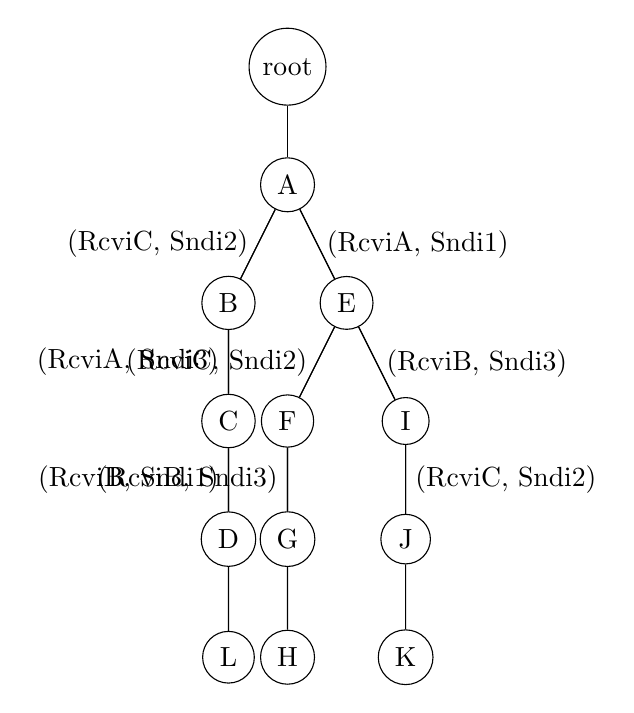
\begin{tikzpicture}
   \tikzstyle{every node}=[circle,draw]
\node(root) {root}
  child{ node(A) {A}
        child{node(B) {B} child{node(C) {C} child{node(D){D} child{node(L){L}}}}}
        child{node (E) {E} 
                child{node(F){F} child{node(G){G} child{node(H){H}}}}
                child{node(I){I} child{node(J){J} child{node(K){K}}}}}};

\tikzstyle{every node}=[->]
\path
(root) edge node[right]{} (A)
(A) edge node[left]{(RcviC, Sndi2)} (B)
    edge node[right]{(RcviA, Sndi1)} (E)
(B) edge node[left]{(RcviA, Sndi3)} (C)
(C) edge node[left]{(RcviB, Sndi1)} (D)
(E) edge node[left]{(RcviC, Sndi2)} (F)
    edge node[right]{(RcviB, Sndi3)} (I)
(F) edge node[left]{(RcviB, Sndi3)} (G)
(I) edge node[right]{(RcviC, Sndi2)} (J);

\end{tikzpicture}
\end{comment}
\caption{An example of Depth-first Search Tree for the CTP}
\label{fig:search_tree}
\end{figure}


\subsection{Overapproximated Match-pair Generation}

Other than simulating all possible executions of the CTP, the algorithm that generates the Overapproximated match pairs is basically a strategy of matching and pruning among all possible Sndi and Rcvi commands with matched end points. We continue using the structure of the lists of Sndi and Rcvi in \figref{fig:data-structure-pendinglist}. The difference is that we do not need to keep multiple copies of both lists for backtracking. We only keep one copy of both lists and store the Rcvi and Sndi commands as follows: The Rcvi commands in all threads are scanned and stored in the list of Rcvi, where the index of a Rcvi command, $r_i$, is the actual order in the thread where this Rcvi command exists. For example, $Rcvi(t_0, i)$ represents the $i_{th}$ Rcvi command in Thread $t_0$. Similarly, the Sndi commands in all threads are stored and ordered in the list of Sndi, where $s_i$ is the index of a Sndi command in the sublist of Sndi commands with same from-end-point and to-end-point. For example, $Sndi(t_0, t_1, j)$ represents the $j_{th}$ Sndi command sending from $t_1$ to $t_0$. In addition, we have the following lemma that supports the pruning strategy in the algorithm.

\begin{lemma}
For each Rcvi command with index $r_i$ and all matched Sndi commands of this Rcvi command, if $s_j$ is the index of any Sndi commands,
\begin{itemize}
\item[1.] $r_i \geq s_j$;
\item[2.] $r_i \leq s_j + (N - sendsize_j)$.
\end{itemize}
Where $N$ is the number of Sndi commands in all threads, and $sendsize_j$ is the size of the sublist where this Sndi command exists.
\label{lemma:Rcvi_Sndi_index}
\end{lemma}
\begin{proof}
We prove it by contradiction. Suppose statement $1$ is not satisfied for some match pair $(Rcvi, Sndi)$, so $r_i < s_j$. Since the Sendi commands with the same from-end-point and to-end-point are sent in a FIFO way, where the first Sndi command should be served first in the destination thread. It is impossible for any strategy to match all those Sendi commands with index less than $s_j$ with some commands because there exist at least one extra Sndi command that can not match any Rcvi command with index less than $r_i$. The contradiction occurs. Thus, statement $1$ is proved.

Similarly, Statement $2$ is not satisfied implies that $r_i > s_j + (N - sendsize_j)$ for the match pair $(Rcvi, Sndi)$. $(N - sendsize_j)$ represents the size of all Sndi commands with from-end-point $j$ and to-end-point other than i. Because of the same reason in the last paragraph, we can not find a strategy that match all Sndi commands with index large than $s_j$ sending from thread $j$ to thread $i$. Thus, the contradiction occurs and statement $2$ is proved.

\end{proof}

The algorithm that generates the overapproximated set of match pairs works as follows:
\begin{itemize}
\item[1] For each Rcvi command $Rcvi(t_s, i)$, all Sndi commands in the entire set of sublists $SndiList(t_s)$ are selected as candidates for matching the Rcvi command.
\item[2] For each candidate Sndi command $Sndi(t_s, t_d, j)$, check if \lemmaref{lemma:Rcvi_Sndi_index} is satisfied. If it is satisfied, the pair $(Rcvi(t_s, i), Sndi(t_s, t_d, j))$ is added to the result set of match pairs. Otherwise, this pair is ignored, and other candidate Sndi commands for $Rcvi(t_s, i)$ are checked.
\item[3] Repeat step 1 and 2 until each Rcvi command is checked with all its candidate Sndi commands.
\end{itemize}

The generated set of match pairs is an overapproximation of the precise set because it contains all legal match pairs. Furthermore, the pruning strategy restricts the size of the set because some match pairs that can illegally occur are removed.

Now, we analyze the time complexity of both algorithms presented in the previous sections. The modified depth first search approach relies on the process of generating and updating the nodes(states) of the search tree, thus, the time complexity is $O(b^N)$, where $b$ is the branching factor. The variation of the branching factor $b$ depends largely on the structure of the CTP. For example, the search tree in \figref{fig:search_tree} can be compressed if the program orders of commands in the scenario are changed. The second algorithm presented above requires several steps to complete. Organizing the contents of pending lists requires linearly scanning the CTP so that the time complexity for this step is $O(N)$. Matching the possible Sndi commands with the given Rcvi commands requires $N_0^2 + N_1^2 + ... + N_n^2 < N^2$ steps, where $N_0 + N_1 + ... + N_n = N$, so this step requires $O(N^2)$ time complexity. Thus, the algorithm that generates the overapproximation of the set of match pairs requires $O(N^2)$ time complexity totally.

\subsection{Stuff needs to be modified}
\begin{itemize}
\item In fist paragraph, how do we claim that an overapproximated set of match pairs is useful? 
\item The figure of the example search tree needs to be modified.
\item Do we need to explain the example tree?
\item The figure of the structure of pending lists should be modified. How to write the math expression in the box?
\item Is the analysis of the time complexity correct?    
\end{itemize}

\section{Related Work}
Morse et al. provided a formal modeling paradigm that is callable from C language for the MCAPI interface \cite{morse:vmcai12}. This model correctly captures the behavior of the interface and can be applied for model checking analysis for C programs that use the API.

In \cite{sharma:fmcad09}, Sharma et al. provided MCC, a dynamic verifier for MCAPI programs. MCC systematically explores all interleavings of an MCAPI program by concretely executing the program repeatedly. MCC also uses DPOR \cite{flanagan:popl05} to reduce the redundant interleavings of the execution. Wang et al. provided a symbolic algorithm that detects errors in all feasible permutations of statements in an execution trace in the shared memory system \cite{wang:fse09}. In this method, the program is partitioned into several concurrent trace programs (CTPs), and the encoding for each CTP is verified using a satisfiability solver. Elwakil et al. provided a similar work with ours \cite{elwakil:atva10,elwakil:padtad10}. In their work, the method of \cite{wang:fse09} is used and adapted to the message passing system. As shown in the previous section of this paper, their method, however, does not correctly encode all possible execution traces of an MCAPI program. 

The application of static analysis is another interesting avenue of research to test or debug message passing programs. \cite{zhang:ppopp07} and \cite{greg:cgo09} are the approaches for MPI \cite{mpi}, another message passing interface standard. \cite{gray:lctes11} presented a system that uses static analysis to determine offline the topology of the communications and nodes in the input MCAPI program.

\section{Conclusions and Future Work}
We have presented an SMT encoding of an MCAPI program execution that uses match pairs rather than the state-based or order-based encoding in the prior work. Unlike the existing method of SMT encoding, our encoding is the first encoding that correctly captures the non-deterministic behaviors of an MCAPI program execution under infinite-buffer semantics allowed in the MCAPI specification. In this paper, we proved that we can generate such an encoding by giving an execution trace and a complete set of match pairs. Further, we have proved that the same results can be obtained even if the match pairs are over-approximated as input. Also, we have provided an algorithm with $O(N^2)$ time complexity that over-approximates the true set of match pairs, where $N$ is the total number of code lines of the program. By comparing to the existing work in \cite{elwakil:padtad10} for a set of ``toy" examples under zero-buffer, our encoding is capable of capturing correct behaviors of an MCAPI program execution and providing efficient solutions. As for the experiment results, we have demonstrated that our encoding scales well for programs with large number of messages and numerous match pairs under infinite-buffer semantics. Also, zero-buffer semantics can be adapted if required.

The precision of the set of match pairs is essential to the efficiency of SMT encodings. Currently we have an over-approximated generation method which still keeps several ``bogus" match pairs in the generated set. New methods for generating a much more precise set of match pair are required. Also The method of DPOR are considered to combine with our SMT encoding to generate the execution traces. We can then use the SMT encoding to further improve the DPOR technique.


\section{Future Work}
The generation of the set of match pairs is essential to the efficiency of our \textit{CEGAR} loop. Currently we have an over-approximated generation method, but the efficiency is not impressive. New methods for generating a much more precise set of match pair are required. 

\bibliographystyle{splncs03}
\bibliography{../bib/paper}
\end{document}
